\documentclass{mpaper}
\usepackage{url}
\usepackage{color}
\usepackage{graphics,graphicx}
\usepackage{epsfig}
\usepackage{epstopdf}
\usepackage{colortbl}
\usepackage{multirow}
\usepackage{booktabs}
\usepackage{ifthen}  
\usepackage{rotating}
\usepackage{tabularx}
\usepackage{subcaption}
\usepackage{varwidth}
\usepackage[labelfont=bf]{caption}
\usepackage[numbers]{natbib}

% This guff allows for tables with line breaks! Use L, C or R as the column type.
\usepackage{array}
\usepackage{ragged2e}
\newcolumntype{L}[1]{>{\raggedright\let\newline\\\arraybackslash\hspace{0pt}}m{#1}}
\newcolumntype{C}[1]{>{\centering\let\newline\\\arraybackslash\hspace{0pt}}m{#1}}
\newcolumntype{R}[1]{>{\raggedleft\let\newline\\\arraybackslash\hspace{0pt}}m{#1}}
\newcolumntype{W}[1]{>{\centering\arraybackslash}m{#1}}

\pagenumbering{arabic}

\begin{document}
\newcommand{\todo}[1]{\textcolor{red}{#1}}

\title{Improving Site Search with Clickthrough Data:\\A Simulated Analysis}
\author{David Maxwell}
\matricnum{0800660}
\maketitle

\begin{abstract}
Today, all major organisations have a presence on the World Wide Web. These websites typically host thousands of pages of content, and often provide a form of search functionality. This functionality acts as a fast and direct way for customers to find the information they are looking for to satisfy their information need. In this paper, we examine the problem of site search, focusing specifically on how organisations can incorporate usage data - as web search engines currently do - in order to improve retrieval quality. To this end, we propose three different ways to incorporate clickthrough data with a standard retrieval function. We then conduct a simulation generating clickthrough data to examine how the quantity and quality of the data affects retrieval performance. Our results show that with a large volume of low-noise clickthrough data, potential performance improvements are large. However, more realistic settings shows a modest improvement in performance. An increase of P@10 from 0.2 to 0.4 requires almost 2000 iterations where there is a high probability of clicking on a relevant item (0.64), and a low probability of clicking on irrelevant items (0.39).
\end{abstract}

%!TEX root = sigir2013site_clicks.tex
\section{Introduction}\label{sec_introduction}
Today, it is uncommon to find an organisation without a presence on the \emph{World Wide Web (Web)}. With many organisations hosting thousands of pages of content, site administrators typically deploy some sort of search functionality to help users find relevant information. Restricted to the content hosted by the organisations in question, such search engine functionality can be defined as \emph{site search}.

Users of site search systems differ depending on the site that is being visited. Users of a governmental website for example may be interested in finding information related to tax returns and driving licences. Users of an academic institution's website may wish to find information about degree programmes the institution is offering. Studies of user behaviour on site search engines have shown that users issue queries which are constrained to the topics encompassed by the organisation in question, with many similar queries are repeated \cite{chau2005site_log_analysis}. This repetitive nature therefore allows us to gather implicit feedback and collate it together to improve performance.

In contrast to site search, \citeauthor{chau2005site_log_analysis} \cite{chau2005site_log_analysis} defines \emph{Web search} as a general-purpose search engine, unrestricted to a particular domain or specialty. Such search engines - such as \emph{Google}\footnote{\url{http://www.google.com}} and \emph{Bing}\footnote{\url{http://www.bing.com}} - each have a wide-ranging index, consisting of billions of documents. This large index may present challenges keeping the index comprehensive and up-to-date, which could potentially lead to results with low precision and recall. \citeauthor{henzinger2002challenges_in_web_search} \cite{henzinger2002challenges_in_web_search} presents a series of further challenges faced by Web search engines. These include dealing with high volumes of spam, wildly varying levels of content quality, and the disregarding of particular `web conventions' by administrators of different sites. Despite Web search engines attempting to cater for a very large and diverse population of users, such search engines generally perform better than site search - a seemingly more constrained problem.

This issue can be attributed to the fact that site search systems have inherent operational challenges which reduce their retrieval performance \cite{ding2007log_based_site_search}. Organisations typically do not have the resources available to investigate means of improving their site search deployment. The organisation may also lack the technical skills to interpret usage data of their search engine. This is compounded by the fact that site search will generate a smaller volume of usage data when contrasted to Web search engines. The smaller volume of usage data could potentially reduce retrieval effectiveness if the data were used to evaluate or tune the search engine.

In its current guise, site search is therefore typically inadequate for a majority of websites that employ it \cite{ding2007log_based_site_search, xue2002log_mining}. It has been argued that search logs could be used to improve site search performance \cite{guo2009click_chain, joachims2002optimizing_clickthrough}. In particular, clickthrough data - which has been successfully leveraged by Web search engines - could be extracted from these logs, and are regarded as a good feature on determining how relevant documents are in relation to a given query \cite{joachims2005clickthrough}.

In this paper, we propose three simple models that combine readily-available clickthrough data with a baseline ranking function with the aim of improving site search performance. We then investigate the behaviour of clickthrough data by performing a series of simulations. These simulations vary the levels of noise and biases which real-world clickthrough data exhibits. We then discuss our findings in detail.

The remainder of this paper is organised as follows. Section \ref{sec_background} reviews related works in the areas of improving the performance of site search, and how clickthrough data has been used. Section \ref{sec_method} presents our research questions, our devised clickthrough models and an overview of our simulations. Section \ref{sec_results} presents our results, while section \ref{sec_conclusion} discusses and concludes the work.
%!TEX root = sigir2013site_clicks.tex
\section{Background}\label{sec_background}
This section details key works in improving the performance of site search engines by incorporating a variety of different features. This section also provides an overview of works that have utilised clickthrough data for various means.

\begin{figure*}
	\begin{center}
	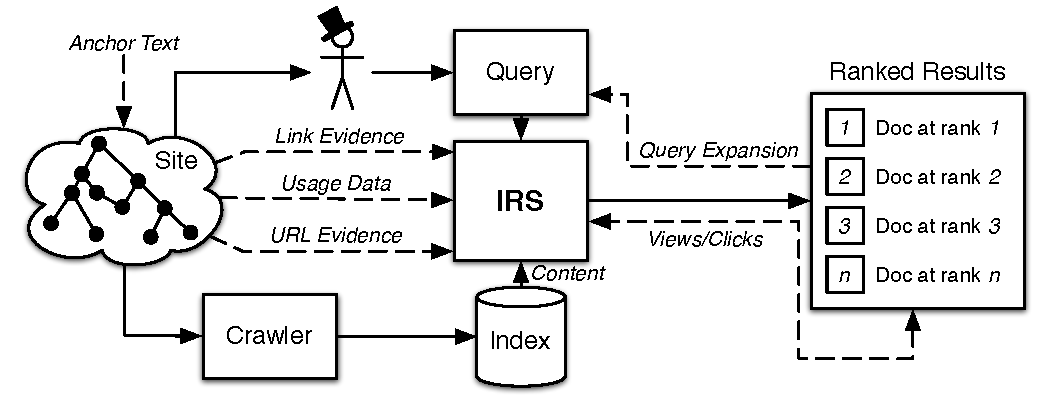
\includegraphics[scale=1.0]{pics/ir_system_new.pdf}
	\end{center}
	\caption{\label{fig:background_architecture}\textbf{A diagram illustrating the basic component architecture of a basic site search system - combined with the different features which have been examined in previous research highlighted in \emph{italics}.\vspace{-0.1cm}}}
\end{figure*}

Today, there are typically three main approaches in which an organisation can deploy site search functionality to their publicly-facing website, intranet, or both. The approaches are:

\begin{itemize}
	
	\item{\textbf{third-party search functionality:} where a commercial Web search engine offers its services for site search;}
	
	\item{\textbf{database driven search:} where an organisation's \emph{Content Management System (CMS)} may provide a SQL-driven search engine, highly unsuitable to semi-structured Web content; and}
	
	\item{\textbf{full-text search engines: } a far superior choice using state-of-the-art technology, with many open-source toolkits in existence for this intent.}
	
\end{itemize}

For the purposes of this paper, we focus exclusively on improving performance of full-text search engines deployed specifically for site search.

\subsection{Improving Site Search}
It is a well recognised problem that the performance of many custom site search engines fall short of the expected standard set by today's modern Web search engines - especially in terms of retrieval accuracy \cite{ding2007log_based_site_search}. Despite the differences in performance, the overall architecture of site search engines are broadly similar to that of a Web search engine - and in turn, a traditional information retrieval system \cite{croft2009search_engine_book}. A diagram depicting the basic architecture of a site search engine can be seen in Figure \ref{fig:background_architecture}, complete with a series of annotations representing features that have been exploited with the aim of improving site search performance. Features examined include: \emph{content}, \emph{link evidence}, \emph{anchor text}, \emph{URL evidence}, \emph{query expansion} and \emph{usage data} (including clickthrough data). It can be noted that many of these techniques have been borrowed from Web search, such are the similarities of the two approaches. In this section, we review research that specifically considers or applies the aforementioned techniques in the context of site search.

Link evidence has been widely exploited by many - if not all - modern Web search engines \cite{upstill2003queryindependent_evidence}, and is considered a powerful approach to improving search performance \cite{carriere1997webquery}. This claim is suitably demonstrated by the \emph{PageRank} algorithm \cite{page1999pagerank}, a cornerstone to Google's success. \citeauthor{carriere1997webquery} \cite{carriere1997webquery} used their \emph{WebQuery} system to examine links amongst documents returned for a given query. The documents with the greatest degree of inlinks were considered ``hot spots'', or documents considered relevant to users. Link evidence was also used by \citeauthor{upstill2003queryindependent_evidence} \cite{upstill2003queryindependent_evidence} in a homepage finding task. Using one enterprise crawl and the TREC WT10G and VLC2 collections, the technique was compared to other forms of query-independent evidence, including \emph{URL-type}, PageRank and anchor text baselines. Their findings showed that more than one form of heuristic should be used in conjunction with link evidence. 

Anchor text has also been examined independently. \citeauthor{fagin2003searching_workplace_web} \cite{fagin2003searching_workplace_web} conducted a study on the IBM intranet where several heuristics were used. Those included were PageRank, inlinks, crawl dates and URL evidence. The use of PageRank and anchor text were considered ``extremely valuable for intranet search'', improving the quality of results returned. They also found the intranet to be jargon-heavy, with users unaware of this. The authors hypothesised that such an issue would hold across other intranets. \citeauthor{upstill2003queryindependent_evidence} \cite{upstill2003queryindependent_evidence} reiterated the findings of \citeauthor{fagin2003searching_workplace_web} \cite{fagin2003searching_workplace_web}, determining that PageRank and anchor text in combination provided an improvement to site search, but may not have been satisfactory by themselves. \citeauthor{hawking2004link_site_search} \cite{hawking2004link_site_search} complemented these findings. While they found improvements in retrieval performance when utilising anchor text from within an organisation's website/intranet, anchor text from external sources was found to be superfluous to improving performance. This finding was used as part of the study by \citeauthor{ding2007log_based_site_search} \cite{ding2007log_based_site_search}, who disregarded any evidence from external documents for the site they were examining. However, \citeauthor{upstill2003queryindependent_evidence} \cite{upstill2003queryindependent_evidence} claim that utilising anchor text from external sources would complement site search due to the smaller collection of documents websites possess compared to the larger Web.

Usage data - in the form of server logs - has been also exploited by many, with server logs described by \citeauthor{guo2009click_chain} \cite{guo2009click_chain} as a ``gold mine'' of information. Such information can be used to help augment site search performance \cite{ding2007log_based_site_search}, and are under the ownership of a website's owner, removing any legal or financial barriers for access \cite{cui2005web_logs_site_search}. \citeauthor{xue2002log_mining} \cite{xue2002log_mining} used server log analysis to improve performance through use of generalisation rule mining. This approach included a hierarchical taxonomy of a given website. The authors then reranked documents by incorporating the taxonomy and prior user behaviours to yield a 15\% improvement over an unspecified ``full-text search'' approach. \citeauthor{cui2005web_logs_site_search} \cite{cui2005web_logs_site_search} constructed a probabilistic graph from log analysis and calculated a new score, \emph{LPageRank}, from webpages within Eastern Kentucky University's domain. The score combined traditional PageRank with other factors, such as the previous number of visits and traffic access patterns. Their results outperformed a traditional PageRank baseline. Finally, \citeauthor{ding2007log_based_site_search} \cite{ding2007log_based_site_search} improved site search performance using a novel approach consisting of two separate indexes. A content-based index, extracted from URLs in server logs, was combined with an anchor-based index. Results showed a maximum performance increase of 22.8\%.

Query expansion has been used by \citeauthor{albakour2012query_reformulations_local} \cite{albakour2012query_reformulations_local}, who performed a study examining query reformulations from a university website. Analysis of query logs showed users were successfully able to reformulate their queries. Clickthrough data was also used as a metric to help identify useful query reformulations. \citeauthor{kruchwitz2013query_suggestions} \cite{kruchwitz2013query_suggestions} also recently conducted a study on different query modification techniques with data collected from site search logs. They found that clustering queries together based upon individual search sessions commonly produced relevant query suggestions.

\subsection{Clickthrough Data - Uses and Issues}\label{sec:background_clickthrough}
Clickthrough data has been exploited for a variety of different purposes. As a form of \emph{implicit relevance feedback}, clickthrough data can be theoretically generated in unlimited volumes \cite{joachims2002optimizing_clickthrough}, but is subject to adverse qualities such as noise and bias \cite{kelly2004time_implicit}. Despite this, clickthrough data is still regarded as a reliable form of implicit feedback \cite{joachims2005clickthrough} and is easy to collect in a non-laboratory setting.

\citeauthor{joachims2005clickthrough} \cite{joachims2005clickthrough} conducted a user study investigating the reliability of clickthrough data as a form of implicit feedback. Two types of analysis were conducted. Eyetracking was recorded to examine how users interacted with a Google results page, the findings of which were compared against \emph{explicit relevance judgements}. Results showed relative preferences were ``reasonably accurate on average'', but also showed a user's clicking habits were intrinsically biased in two ways. \emph{Positional bias} showed that users trusted the retrieval method used by only clicking on documents high in the rankings. This behaviour was also observed by \citeauthor{granka2004eyetracking} \cite{granka2004eyetracking}. A \emph{quality bias} also showed that clicking behaviour was not only influenced by the relevance of a clicked link, but also by the overall quality of the other abstracts for surrounding documents.

Many techniques used to evaluate the reliability of clickthrough data use explicit relevance judgements, or \emph{editorial judgements}. However, an organisation wishing to improve their site search offering would likely not be able to afford or attain such judgements for their documents. \citeauthor{dupret2010intrinsic_document_relevance_clickthrough_logs} \cite{dupret2010intrinsic_document_relevance_clickthrough_logs} devised the \emph{Cumulative Relevance Model}, based upon explicit assumptions of a user's behaviour. These assumptions accounted for his or her actions throughout a search session, which was considered successful if it ended with a click on a ranked document. The model proved useful for sessions with low click rates - an inherent problem of site search. \citeauthor{hofmann2011graded_relevance} \cite{hofmann2011graded_relevance} showed how judgements obtained from clickthrough data could be evaluated.

Studies have also focused on how clickthrough data can improve search performance, such as those by \citeauthor{agichtein2006improving_web_search} \cite{agichtein2006improving_web_search} and \citeauthor{xue2003web_logs_site_search} \cite{xue2003web_logs_site_search}. In \cite{agichtein2006improving_web_search}, clickthrough data was incorporated using a machine-learned function, and was demonstrated to outperform competitive Web search ranking algorithms by as much as 31\%.
%!TEX root = sigir2013site_clicks.tex
\section{Experimental Method}\label{sec_method}
Studies suggest that in recent years, there has been a shift towards using machine learning techniques and clickthrough data to improve search engine performance. While the benefits of such approaches are evident, the technique leaves a knowledge gap in understanding exactly how the behaviour of clickthrough data changes by varying associated aspects.

This section outlines a series of devised models that incorporate clickthrough data and associated evidence into document scorings and rankings. We also provide the key research questions we wish to address, our baseline setup details, and information on our clickthrough simulator. The section is concluded with a high-level description of our devised simulations.

\subsection{Research Questions and Hypotheses}\label{sec:method:questions}
The main objective of this study was to investigate \emph{by how much clickthrough data can improve the performance of site search} and \emph{how clickthrough data could be incorporated}. Specifically, we examined how much data was required, and what conditions were required to achieve performance increases. These issues can be represented by the following research questions: 

\begin{enumerate}
	
	\item{\emph{Of what quality does clickthrough data need to possess to yield good results?} A single click can only be considered as a weak indicator of relevance \cite{kelly2005implicit_feedback}. As such, clickthrough data, like other forms of implicit feedback, is considered noisy. As such, a quality threshold must be determined - if this level is reached or exceeded, retrieval performance will begin to fall.}
	
	\item{\emph{What trade-offs are there regarding quality of data and quantity?} Taking into account both the quantity and quality of clickthrough data, are there any links between the two which could be exploited to reach the highest performance level attainable?}

\end{enumerate}

To study this problem, we modelled a series of clickthrough simulations. Simulations allow researchers to conduct carefully designed and controlled experiments. From these, precise answers to research questions can be obtained \cite{azzopardi2011economics_of_iir, white05sim}. Our simulations therefore provided us with the necessary control to obtain an understanding of the influence clickthrough data had on performance.

\subsection{Data and Materials}\label{sec:method:materials}
For this study, we used the TREC \emph{DOTGOV1} collection. The collection comprises of 1,247,753 documents, and was used in conjunction with TREC topic 551-600 and their associated explicit relevance judgements. The DOTGOV1 collection is a compilation of crawled documents across the US Government's TLD, \texttt{.gov}.

The collection was indexed with the \emph{Indri}\footnote{\url{http://www.lemurproject.org/indri.php}} toolkit, which is part of the \emph{Lemur}\footnote{\url{http://www.lemurproject.org/}} project. It was preprocessed in four ways to create four individual inverted indexes. The combinations used were: indexing with stopwords removed\footnote{We used Fox's classical stopword list \cite{fox1992lexical_analysis}, containing a total of 733 stopwords.}, indexing with Porter stemming applied, indexing with both stopword removal and Porter stemming applied, and without any preprocessing whatsoever.

We then ran the TF-IDF, PL2 and BM25 retrieval models over each created index, varying the $\beta$ and $c$ values for the BM25 and PL2 models respectively. For $\beta$, variations in steps of 0.1 were evaluated between 0.0 and 1.0. For $c$, variations in steps of 1.0 between 1.0 and 10.0 were evaluated. For the DOTGOV1 index, the BM25 retrieval model with Porter stemming offered the highest performance values, and was thus selected to act as the baseline system for our work. Performance values across all four indexes created with the BM25 retrieval model are summarised in Table \ref{tbl:baselines}.

\begin{table}[h]
	\renewcommand{\arraystretch}{1.3}
	\begin{center}
		\begin{small}
			\begin{tabularx}{\linewidth}{X|c|c|c|c}
				\textbf{\emph{Variant}} & \textbf{\emph{$\beta$}} & \textbf{\emph{MAP}} & \textbf{\emph{P@5}} & \textbf{\emph{P@10}}
				\tabularnewline
				\hline
				N/A & 0.6 & 0.1689 & 0.248 & 0.212 \tabularnewline \hline
				\textbf{Porter} & \textbf{0.6} & \textbf{0.1842} & \textbf{0.272} & \textbf{0.226} \tabularnewline \hline
				Stopword & 0.6 & 0.1674 & 0.248 & 0.212 \tabularnewline \hline
				Stopword + Porter & 0.6 & 0.1786 & 0.264 & 0.216 \tabularnewline
			\end{tabularx}
		\end{small}
	\end{center}
	
	\vspace{-0.4cm}
	\caption{\textbf{Table illustrating the different performance values obtained using the BM25 model across the four preprocessed variants of the DOTGOV1 collection. The highest performance values (selected as our baseline) are highlighted in bold.}}
	\label{tbl:baselines}
\end{table}

Although for the purposes of this work the baseline value is not altogether that important, it is nevertheless good practice to select a modest baseline from which to improve. Across IR research, BM25 has been widely used as a baseline for experimentation (see \cite{moon2010user_driven_ranking} and \cite{upstill2003queryindependent_evidence} for examples).

\subsection{Combining Evidence}
To incorporate clickthrough data evidence into the scoring of documents, we used a simple, aggregative technique based on the \emph{combSUM} approach defined by \citeauthor{shaw1993combining} \cite{shaw1993combining}. The technique can be represented by the function $S(q, d)$:

\vspace{-0.3cm}
\begin{equation}
	S(q, d) = bs_q(d) + C_q(d)
\end{equation}

\noindent
where $q$ is a given query/topic, and $d$ is a document ranked in that query's results; $bs_q(d)$ is the baseline score for the given query/document combination; and $C_q(d)$ is some function which incorporates clickthrough data evidence. Section \ref{sec:method:models} details the models that were devised that incorporate clickthrough data.

\subsection{Clickthrough Models}\label{sec:method:models}
Here, we describe the three models that were developed as part of this study which incorporate clickthrough data and other forms of related evidence. The models can be broadly split into two categories, with one \emph{promotion-only} model, and two \emph{promotion and demotion} models. The terms promotion and demotion relate to the promotion and demotion of documents in document rankings when clickthrough data are considered.

To express the models in a simple form, we use the following nomenclature in their descriptions. Note that all mentions of a document, $d$, must be considered in relation to a user's query, $q$.

\begin{itemize}
	
	\item[$R_d$]{The current rank of document $d$.}
	
	\item[$N_d$]{The number of times document $d$ has been displayed in the top-$k$ of a query's results, where $k$ is the depth of a given simulation (see Section \ref{method:simulator:clickthrough}).}
	
	\item[$E_d$]{The number of aggregated examinations that document $d$ has received from simulated users.}
	
	\item[$C_d$]{The number of aggregated clicks that document $d$ has attracted from simulated users.}
	
	\item[$\overline{C_d}$]{The number of times that document $d$ has \emph{not} been clicked when it was visible to a simulated user. Thus, $\overline{C_d} = N_d - C_d$.}
	
\end{itemize}

\subsubsection{Promotion-Only Model}\label{sec:method:models:promo}
Our simple promotion-only model uses a multiplicative approach to combine clickthrough evidence. Abbreviated as model \textbf{P} throughout this paper, the model can be defined thus:
\vspace{-0.1cm}
\begin{equation}
	C_q(d) = \alpha C_d
	\label{eqn:p}
\end{equation}

\noindent
where $\alpha$ is a tuning parameter, used to adjust the weighting of clickthrough evidence in document scoring.

Given this formulation, it is clear that if we have `perfect' clickthrough data - where users click only on relevant documents - this model will percolate relevant documents upwards at a rate of $\alpha$. However, as noise is introduced, as long as the proportion of relevant documents clicked is higher than the number of non-relevant documents clicked, then relevant documents should percolate up the rankings. A point existed where this was no longer the case - it is this point which we wished to find empirically.

\subsubsection{Promotion and Demotion Models}
We also devised two further models that demote documents as well as promote. Behind this concept is the belief that if irrelevant documents can be demoted, relevant documents will percolate to the top of the rankings faster than when compared to a promotion-only approach.

We devised a simple promotion/demotion model that promotes documents based on the number of clicks a document receives. Additionally, the model demotes those documents that are clicked on infrequently. The model is abbreviated as \textbf{PD} in this paper.
\vskip -0.3cm
\begin{equation}
	C_q(d) = \alpha C_d - \beta \overline{C_d}
	\label{eqn:pd}
\end{equation}

The model, like \textbf{P} shown in Equation \ref{eqn:p}, uses tuning parameter $\alpha$ to influence the weighting of promoting documents. The promotion/demotion model also includes an additional tuning parameter, $\beta$, for influencing the weighting of demoting documents. While the issue of demoting documents may be addressed, model \textbf{PD} may not be particularly robust to noisy clickthrough data - or scenarios where relevant documents are not clicked. These are considered in our final model.

Abbreviated as \textbf{PDE} in this paper, our final model also includes the tuning parameters as mentioned for model \textbf{PD}. For this model, we also include two key features of clickthrough data: the examination hypothesis \cite{craswell2008click_position_bias_models}, and positional bias.
\vspace{-0.1cm}
\begin{equation}
	C_q(d) = \alpha C_d - \left[\frac{\beta(E_d - C_d)}{R_d}\right]
	\label{eqn:pde}
\end{equation}

For this model, we assume that the number of clicks a document receives subtracted from the number of examinations it receives provides an indicator of how irrelevant a document is to a given query. This means that an infrequently clicked document is more likely to be demoted down the rankings. We also make this score proportional to the rank at which a document is currently at: this adds the concept of positional bias.

\subsubsection{Clickthrough Modelling in Prior Works}
Several studies have proposed different approaches to modelling clickthrough data which are not used in this paper. \citeauthor{dupret2008user_browsing_model} \cite{dupret2008user_browsing_model} extended the examination model with the \emph{User Browsing Model} where distances from previously clicked documents are factored into the probability of clicking the next. \citeauthor{craswell2008click_position_bias_models} \cite{craswell2008click_position_bias_models} also introduced the \emph{Mixture Model} - where users would blindly click on highly ranked documents (as if in a rush) - and the \emph{Cascade Model} - where users would scan results from top to bottom in a linear fashion. Several studies since have developed the idea of the Cascade Model to consider further aspects \cite{chapelle2009bayesian, guo2009click_chain, guo2009multiple_click_models}.

\subsection{Clickthrough Simulator}\label{method:simulator:clickthrough}
The devised clickthrough models were implemented as part of our clickthrough simulator\footnote{The clickthrough simulator implemented as part of this study was written in the \href{http://www.python.org/download/releases/2.7/}{\emph{Python}} programming language. The source code is available on request.}. The simulator was extensively used to run a series of simulations of a user's behaviour when interacting with search results. By taking in a set of ranked results (in the case of this study, the previously discussed baselines) and corresponding relevance judgements, the system would simulate user behaviour over a series of iterations. Each iteration of the simulation is analogous to a real-world user of a search engine examining (viewing) a series of ranked documents for several queries, potentially leading to the clicking of document(s) he or she feels is/are relevant to his or her information need.

Simulated interactions could be controlled by a series of customisable parameters to suit individual cases. Parameters included:

\begin{itemize}
	
	\item{a depth parameter, allowing for control of how far down the ranked results list a simulated user would be prepared to look for relevant results;}
	
	\item{a parameter allowing for determining the probability of examining a document, $P(E)$ - which could be proportional to the depth/rank of a given document in the results list, known as the examination model \cite{richardson2007predicting_clicks, craswell2008click_position_bias_models};}
	
	\item{parameters allowing for the adjustment of the probability of a user clicking a relevant document, $P(C|R)$, and the probability of clicking an irrelevant document, $P(C|N)$; and}
	
	\item{the customisation of $\alpha$ and $\beta$ parameters for the devised clickthrough models, as discussed in Section \ref{sec:method:models}.}
	
\end{itemize}

Each iteration produced a series of files, including \texttt{.views} and \texttt{.clicks} files, containing the aggregated number of examinations and clicks that a topic/document pairing had received, respectively. Also included was a \texttt{.topk} file, containing the aggregated number of appearances a document had appeared - in relation to a given query - in the top-$k$ of the ranked results. $k$ denoted the depth of a given simulation. Of particular importance was the file containing a new set of results, which combined clickthrough evidence to produce new document scores. With each results file generated, the simulation's performance after each iteration could be evaluated with a tool such as \href{http://trec.nist.gov/trec_eval/}{\texttt{trec\_eval}}.

By evaluating performance after each iteration, we could compare the MAP of iteration $i-1$ against the MAP of iteration $i$. This comparison was to ensure that the performance had not converged or fallen. If either case was reached, and no further improvement in MAP was noted after 200 iterations, the simulation was deemed complete and then stopped. For the purposes of our simulations, we ran to a maximum of 1000 iterations - or the last increase in MAP + 200 iterations, whichever came first.

\subsection{Clickthrough Simulations}\label{method:simulations}
With our three models devised, we developed a number of simulations to evaluate each model's performance across a range of different simulation parameters, which are enumerated in Section \ref{method:simulator:clickthrough}. Of particular interest was determining values for the $\alpha$ and $\beta$ parameters, controlling the weighting of document promotion and demotion respectively.

Our approach included:

\begin{itemize}
	
	\item{a series of simulations that examined the behaviour of clickthrough data in `perfect' conditions, free of bias and noise, (with $P(C|N) = 0.0$);}
	
	\item{simulations that examined the impact on performance when positional bias was included (when $P(E)$ was varied);}
	
	\item{simulations that examined performance when `noisy', imperfect data was introduced (with variations in both $P(C|R)$ and $P(C|N)$); and}
	
	\item{simulations that examined performance with probabilities obtained from a recent user study (see \cite{smucker2012time_based_calibration}, where we obtain realistic values for $P(C|R)$ and $P(C|N)$).}
	
\end{itemize}

The setup for each simulation - as well as a discussion on the results obtained from each - can be found in Section \ref{sec_results}.
%!TEX root = sigir2013site_clicks.tex
\section{Analysis and Results}\label{sec_results}
In this section, we present our simulations and discuss our findings from each.

\subsection{A Perfect World}
As a form of implicit relevance feedback, obtaining clickthrough data under ideal conditions - where the collected data are free from any form of noise or bias - is a highly unrealistic goal to aim for in a real-world scenario.

Despite this, data collected in an ideal environment does provide us with a better understanding of the maximum attainable performance improvements that clickthroughs can theoretically provide. As such, examining data collected in ideal conditions allowed us to answer the following operational questions.

\begin{enumerate}
	
	\item{\emph{What is the maximum performance attainable when clickthrough data are incorporated?}}
	
	\item{\emph{How fast can maximum performance be reached?}}
	
\end{enumerate}

We addressed these questions with a series of simulations run across all three devised models. For each model, we set $P(C|N)$ to a 0.0, and vary $P(C|R)$, using the values 0.25, 0.5, 0.75 and 1.0. These settings exhibited the aforementioned `ideal' conditions, ensuring that all clicks are only on relevant documents. We hypothesised that as the probability of clicking on relevant documents is decreased, the number of iterations required to reach a maximum performance threshold increased - but would converge at the same points. We also varied the depth, $d$, of the simulations, using values of 10, 20 and 30. This was to examine whether an increase in depth would yield an increase or decrease in performance.

For the promotion-only algorithm \textbf{P}, we also ran simulations over a range of $\alpha$ values, namely 0.05, 0.1, 0.25, 0.5, 0.75, 1.0 and 2.0. For the demotion algorithms \textbf{PD} and \textbf{PDE}, we selected a value for $\alpha$ that offered good performance for \textbf{P}. However, we varied $\beta$ using the same numerical range.

\subsubsection{Results}
When combining `perfect' clickthrough evidence, we observed performance improvements over our baseline system of some 265\%. For \textbf{P}, a MAP of 0.2774 was attained. For \textbf{PD} and \textbf{PD}, MAP values of 0.6727 and 0.3931 were obtained respectively.

%For promotion-only model \textbf{P}, the results in Table \ref{tbl:results_perfect_multiplicative} provide a summary of our findings. For \textbf{P}, the maximum attainable performance was identical when $\alpha > 0$. When $d=10$, MAP increased from 0.1842 to 0.2188. When $d=20$ and $d=30$, MAP increased even further - to 0.2358 and 0.2774 respectively. The explanation for this behaviour is that as $d$ increases, more documents in the document rankings have a chance to be promoted. $\alpha$, while having no effect on overall performance, does vary the rates at which performance converges. A higher $\alpha$ value results in performance converging in fewer iterations.

%\todo{==========}

\textbf{\emph{What is the maximum performance attainable when clickthrough data is incorporated?}}
Improvements over our baseline across all three clickthrough models. Running each model across our three chosen depths of 10, 20 and 30, we noted that performance increased further the greater the depth. This finding is intuitive, and can be explained by the fact that as the simulation depth increases, more potentially relevant documents will be viewed and clicked, which percolate up the rankings.

\begin{table}[t!]
	\renewcommand{\arraystretch}{1.3}
	\begin{center}
		\begin{small}
			\begin{tabularx}{\linewidth}{W{0.86cm}|W{1.4cm}|W{1.4cm}|W{1.4cm}|W{1.4cm}W{0.00000001cm}}
				
			 	& & \centering{\textbf{\emph{MAP}}} & \centering{\textbf{\emph{P@5}}} & \centering{\textbf{\emph{P@10}}}&
				\tabularnewline
				\hline
				
				\centering{BL}
				& \centering{$\alpha = 0$}
				& \centering{0.1842}
				& \centering{0.2720}
				& \centering{0.2260}&
				\tabularnewline[1em]
				\hline
				
				\multirow{4}{*}{\vspace{-2cm}\hspace{0.18cm}\begin{rotate}{90}$P(C|R) > 0.0$\end{rotate}}
				& \centering{$\alpha > 0$\\$d = 10$}
				& \centering{0.2188}
				& \centering{0.4240}
				& \centering{0.2260}&
				\tabularnewline
				\cline{2-5}
				
				& \centering{$\alpha > 0$\\$d = 20$}
				& \centering{0.2358}
				& \centering{0.5320}
				& \centering{0.3520}&
				\tabularnewline
				\cline{2-5}
				
				& \centering{$\alpha > 0$\\$d = 30$}
				& \centering{\textbf{0.2774}}
				& \centering{\textbf{0.5960}}
				& \centering{\textbf{0.4240}}&
				\tabularnewline
				
				
			\end{tabularx}
		\end{small}
	\end{center}
	
	\vspace{-0.4cm}
	\caption{\textbf{Table illustrating the highest performance levels attained using the promotion-only model. The table shows performance differences across varying simulation depths. \emph{BL} indicates baseline values.}\vspace{-0.2cm}}
	\label{tbl:results_perfect_multiplicative}
\end{table}

\begin{table}[t!]
	\renewcommand{\arraystretch}{1.3}
	\begin{center}
		\begin{small}
			\begin{tabularx}{\linewidth}{W{0.86cm}|W{1.4cm}|W{1.4cm}|W{1.4cm}|W{1.4cm}W{0.00000001cm}}
			 	& & \centering{\textbf{\emph{MAP}}} & \centering{\textbf{\emph{P@5}}} & \centering{\textbf{\emph{P@10}}} &
				\tabularnewline
				\hline
				
				\centering{BL}
				& \centering{$\alpha = 0$}
				& \centering{0.1842}
				& \centering{0.2720}
				& \centering{0.2260} &
				\tabularnewline[1em]
				\hline
				
				\hspace{4cm}P
				& \multicolumn{1}{c|}{\multirow{2}{*}{\begin{varwidth}{1.15cm}\centering{$\alpha=0.75$ $d=30$}\end{varwidth}}}
				& \centering{0.2774}
				& \centering{0.5960}
				& \centering{0.4240} &
				\tabularnewline[1.4em]
				\cline{3-5}
				
				&
				& \multicolumn{3}{c}{$i = 12$}
				\tabularnewline
				
				\hline
				\hline
				
				\multirow{4}{*}{\vspace{-3.45cm}\hspace{0.18cm}\begin{rotate}{90}$P(C|R) > 0.25$\end{rotate}}
				& \multicolumn{1}{c|}{\multirow{2}{*}{\begin{varwidth}{1.15cm}\centering{$\alpha=0.75$ $\beta>0$ $d=10$}\end{varwidth}}}
				& \centering{{\makebox[0pt][c]{{\tiny $\beta@0.05$} 0.4412}\\\makebox[0pt][c]{{\tiny $\beta@2.0$} 0.5140}}}
				& \centering{{\makebox[0pt][c]{{\tiny $\beta@0.05$} 0.8720}\\\makebox[0pt][c]{{\tiny $\beta@2.0$} 0.7160}}}
				& \centering{{\makebox[0pt][c]{{\tiny $\beta@0.05$} 0.8920}\\\makebox[0pt][c]{{\tiny $\beta@2.0$} 0.8100}}} &
				\tabularnewline[1.4em]
				\cline{3-5}
				
				&
				& \multicolumn{3}{c}{$\beta = 0.05, i = 1000$ - $\beta = 2.00, i = 685$}
				\tabularnewline
				\cline{2-5}
				
				& \multicolumn{1}{c|}{\multirow{2}{*}{\begin{varwidth}{1.15cm}\centering{$\alpha=0.75$ $\beta>0$ $d=20$}\end{varwidth}}}
				& \centering{{\makebox[0pt][c]{{\tiny $\beta@0.05$} 0.5732}\\\makebox[0pt][c]{{\tiny $\beta@2.0$} 0.6318}}}
				& \centering{{\makebox[0pt][c]{{\tiny $\beta@0.05$} 0.8880}\\\makebox[0pt][c]{{\tiny $\beta@2.0$} 0.8920}}}
				& \centering{{\makebox[0pt][c]{{\tiny $\beta@0.05$} 0.7940}\\\makebox[0pt][c]{{\tiny $\beta@2.0$} 0.8100}}} &
				\tabularnewline[1.4em]
				\cline{3-5}
				
				&
				& \multicolumn{3}{c}{$\beta = 0.05, i = 1000$ - $\beta = 2.00, i = 381$}
				\tabularnewline
				\cline{2-5}
				
				& \multicolumn{1}{c|}{\multirow{2}{*}{\begin{varwidth}{1.15cm}\centering{$\alpha=0.75$ $\beta>0$ $d=30$}\end{varwidth}}}
				& \centering{{\makebox[0pt][c]{{\tiny $\beta@0.05$} 0.6269}\\\makebox[0pt][c]{{\tiny $\beta@2.0$} 0.6727}}}
				& \centering{{\makebox[0pt][c]{{\tiny $\beta@0.05$} 0.8920}\\\makebox[0pt][c]{{\tiny $\beta@2.0$} 0.8920}}}
				& \centering{{\makebox[0pt][c]{{\tiny $\beta@0.05$} 0.8060}\\\makebox[0pt][c]{{\tiny $\beta@2.0$} 0.8100}}} &
				\tabularnewline[1.4em]
				\cline{3-5}
				
				&
				& \multicolumn{3}{c}{$\beta = 0.05, i = 995$ - $\beta = 2.00, i = 311$}
				\tabularnewline
				\hline
				\hline
				
				\multirow{4}{*}{\vspace{-3.45cm}\hspace{0.18cm}\begin{rotate}{90}$P(C|R) = 0.25$\end{rotate}}
				& \multicolumn{1}{c|}{\multirow{2}{*}{\begin{varwidth}{1.15cm}\centering{$\alpha=0.75$ $\beta>0$ $d=10$}\end{varwidth}}}
				& \centering{{\makebox[0pt][c]{{\tiny $\beta@0.05$} 0.4333}\\\makebox[0pt][c]{{\tiny $\beta@2.0$} 0.1842}}}
				& \centering{{\makebox[0pt][c]{{\tiny $\beta@0.05$} 0.8600}\\\makebox[0pt][c]{{\tiny $\beta@2.0$} 0.2720}}}
				& \centering{{\makebox[0pt][c]{{\tiny $\beta@0.05$} 0.7040}\\\makebox[0pt][c]{{\tiny $\beta@2.0$} 0.2260}}} &
				\tabularnewline[1.4em]
				\cline{3-5}
				
				&
				& \multicolumn{3}{c}{$\beta = 0.05, i = 992$ - $\beta = 2.00, i = 0$}
				\tabularnewline
				\cline{2-5}
				
				& \multicolumn{1}{c|}{\multirow{2}{*}{\begin{varwidth}{1.15cm}\centering{$\alpha=0.75$ $\beta>0$ $d=20$}\end{varwidth}}}
				& \centering{{\makebox[0pt][c]{{\tiny $\beta@0.05$} 0.5668}\\\makebox[0pt][c]{{\tiny $\beta@2.0$} 0.1842}}}
				& \centering{{\makebox[0pt][c]{{\tiny $\beta@0.05$} 0.8880}\\\makebox[0pt][c]{{\tiny $\beta@2.0$} 0.2720}}}
				& \centering{{\makebox[0pt][c]{{\tiny $\beta@0.05$} 0.7840}\\\makebox[0pt][c]{{\tiny $\beta@2.0$} 0.2260}}} &
				\tabularnewline[1.4em]
				\cline{3-5}
				
				&
				& \multicolumn{3}{c}{$\beta = 0.05, i = 1000$ - $\beta = 2.00, i = 0$}
				\tabularnewline
				\cline{2-5}
				
				& \multicolumn{1}{c|}{\multirow{2}{*}{\begin{varwidth}{1.15cm}\centering{$\alpha=0.75$ $\beta>0$ $d=30$}\end{varwidth}}}
				& \centering{{\makebox[0pt][c]{{\tiny $\beta@0.05$} 0.6243}\\\makebox[0pt][c]{{\tiny $\beta@2.0$} 0.1842}}}
				& \centering{{\makebox[0pt][c]{{\tiny $\beta@0.05$} 0.8920}\\\makebox[0pt][c]{{\tiny $\beta@2.0$} 0.2720}}}
				& \centering{{\makebox[0pt][c]{{\tiny $\beta@0.05$} 0.8060}\\\makebox[0pt][c]{{\tiny $\beta@2.0$} 0.2260}}} &
				\tabularnewline[1.4em]
				\cline{3-5}
				
				&
				& \multicolumn{3}{c}{$\beta = 0.05, i = 1000$ - $\beta = 2.00, i = 0$}
				\tabularnewline
				
			\end{tabularx}
		\end{small}
	\end{center}
	
	\vspace{-0.4cm}
	\caption{\textbf{Table summarising the performance values achieved across varying $P(C|R)$ and depth values using the \emph{PD} model, where $\alpha = 0.75$. For brevity, very similar results for $P(C|R) = 0.25$, $P(C|R) = 0.5$ and $P(C|R) = 0.75$ are condensed into $P(C|R) > 0.25$. \emph{BL} indicates baseline values, \textbf{\emph{P}} denotes the best performance achieved using model \emph{P}. Lower $i$ values indicate maximum performance is reached earlier.}\vspace{-0.4cm}}
	\label{tbl:results_perfect_demotive}
\end{table}

Starting with our baseline MAP of 0.1842, our three models improved to maximums of 0.2774, 0.6727 and 0.3931 for models \textbf{P}, \textbf{PD} and \textbf{PDE} respectively - with all values being observed with $d=30$. Tables \ref{tbl:results_perfect_multiplicative}, \ref{tbl:results_perfect_demotive} and \ref{tbl:results_perfect_view} present the maximum performance values obtained across the parameters we varied. To obtain the best performance, it did not matter what value $\alpha$ was assigned. We decided to use $\alpha = 0.75$ for the other two models so as to not dominate their respective demotion aspects.

Of interest is the varying performance levels observed between the three models. With the performance of \textbf{PD} clearly superior to \textbf{P} and \textbf{PDE}, what are the key differences between the models which can account for such a variation?

Compared to \textbf{PD}, model \textbf{P} is promotion-only, meaning that irrelevant documents are not directly demoted. They may however fall down rankings as relevant documents are pushed up, but never at the same rate as a promotion and demotion approach. Model \textbf{PDE} -  while possessing the ability to demote documents - also takes into account the rank at which documents reside. This means that documents at lower ranks are less likely to be promoted, explaining the difference in performance over model \textbf{PD}.

Also important to achieving a high performance is the value of demotion tuning parameter, $\beta$. Too high, the demotion aspect of \textbf{PD} and \textbf{PDE} becomes too aggressive; too low, the demotion aspect is not aggressive enough. By examining Tables \ref{tbl:results_perfect_demotive} and \ref{tbl:results_perfect_view}, it can be seen that the best performance is achieved when $\beta = 2.0$. However, as $P(C|R)$ is decreased, the best performance can be attained with a much smaller $\beta$ value. This can be explained due to the fact that with a lower $P(C|R)$ value, relevant documents are less likely to be clicked. With fewer clicks, documents are more susceptible to demotion.

To examine this phenomenon, we ran a further simulation using \textbf{PD} and set $P(C|R)$ to 0.25. We varied $\beta$ from 0.0 to 2.0. We used steps of 0.01 between 0.0 and 0.25 to obtain a better perspective of performance at lower $\beta$ values.  As shown in Figure \ref{fig:perfect_map_fall}, results show a peak in performance at much lower $\beta$ values - in the range from 0.05 to 0.20. After 0.20, performance begins to drop significantly as the demotion aspect of the \textbf{PD} model becomes too aggressive. In some cases, demotion is so aggressive that performance begins to drop - in some cases \emph{below} our baseline values.
 
\begin{figure}
	\begin{center}
	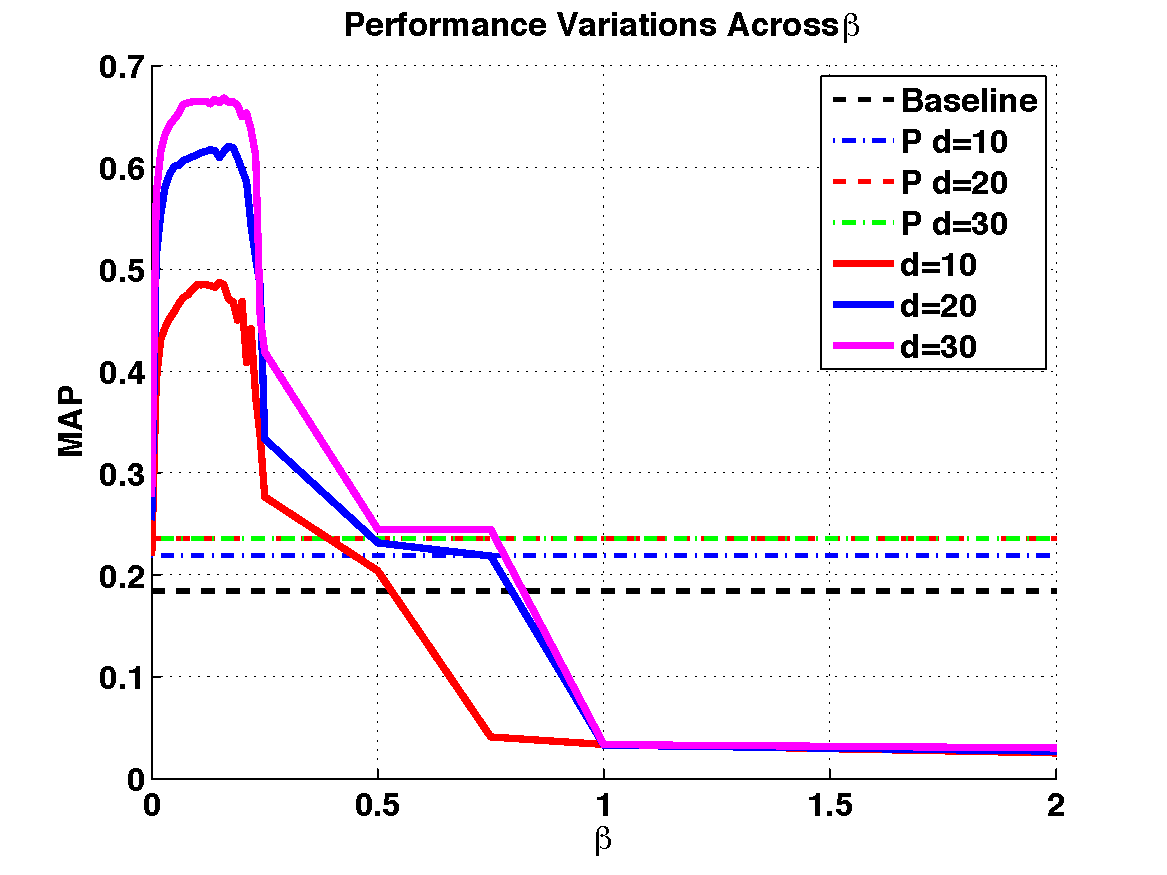
\includegraphics[width=\linewidth]{pics/perfect/perfect_map_fall.pdf}
	\end{center}
	\vspace{-0.5cm}
	\caption{\label{fig:perfect_map_fall}\textbf{A line graph illustrating the significant fall in performance as $\beta$ is increased after 0.25. Data are from the `ideal' simulations for the PD model with $P(C|R) = 0.25$.}\vspace{-0.5cm}}
\end{figure}

\textbf{\emph{How fast can maximum performance be reached?}}
The number of iterations required for performance to reach its maximum varies on a combination of parameters. We varied $P(C|R)$ to specifically examine this issue. For many cases where performance continues to increase with a lower $P(C|R)$ value, several simulations hit our imposed limit of 1000 iterations; we hypothesise that if these were to continue, performance would eventually converge.

\begin{table}[t!]
	\renewcommand{\arraystretch}{1.3}
	\begin{center}
		\begin{small}
			\begin{tabularx}{\linewidth}{W{0.86cm}|W{1.4cm}|W{1.4cm}|W{1.4cm}|W{1.4cm}W{0.00000001cm}}
			 	& & \centering{\textbf{\emph{MAP}}} & \centering{\textbf{\emph{P@5}}} & \centering{\textbf{\emph{P@10}}} &
				\tabularnewline
				\hline
				
				\centering{BL}
				& \centering{$\alpha = 0$}
				& \centering{0.1842}
				& \centering{0.2720}
				& \centering{0.2260} &
				\tabularnewline[1em]
				\hline
				
				\hspace{4cm}P
				& \multicolumn{1}{c|}{\multirow{2}{*}{\begin{varwidth}{1.15cm}\centering{$\alpha=0.75$ $d=30$}\end{varwidth}}}
				& \centering{0.2774}
				& \centering{0.5960}
				& \centering{0.4240} &
				\tabularnewline[1.4em]
				\cline{3-5}
				
				&
				& \multicolumn{3}{c}{$i = 12$}
				\tabularnewline
				
				\hline
				\hline
				
				\multirow{4}{*}{\vspace{-3.45cm}\hspace{0.18cm}\begin{rotate}{90}$P(C|R) = 1.0$\end{rotate}}
				& \multicolumn{1}{c|}{\multirow{2}{*}{\begin{varwidth}{1.15cm}\centering{$\alpha=0.75$ $\beta>0$ $d=10$}\end{varwidth}}}
				& \centering{{\makebox[0pt][c]{{\tiny $\beta@0.05$} 0.2592}\\\makebox[0pt][c]{{\tiny $\beta@2.0$} 0.2869}}}
				& \centering{{\makebox[0pt][c]{{\tiny $\beta@0.05$} 0.5600}\\\makebox[0pt][c]{{\tiny $\beta@2.0$} 0.6520}}}
				& \centering{{\makebox[0pt][c]{{\tiny $\beta@0.05$} 0.3420}\\\makebox[0pt][c]{{\tiny $\beta@2.0$} 0.4320}}} &
				\tabularnewline[1.4em]
				\cline{3-5}
				
				&
				& \multicolumn{3}{c}{$\beta = 0.05, i = 993$ - $\beta = 2.00, i = 1000$}
				\tabularnewline
				\cline{2-5}
				
				& \multicolumn{1}{c|}{\multirow{2}{*}{\begin{varwidth}{1.15cm}\centering{$\alpha=0.75$ $\beta>0$ $d=20$}\end{varwidth}}}
				& \centering{{\makebox[0pt][c]{{\tiny $\beta@0.05$} 0.3068}\\\makebox[0pt][c]{{\tiny $\beta@2.0$} 0.3514}}}
				& \centering{{\makebox[0pt][c]{{\tiny $\beta@0.05$} 0.6560}\\\makebox[0pt][c]{{\tiny $\beta@2.0$} 0.7280}}}
				& \centering{{\makebox[0pt][c]{{\tiny $\beta@0.05$} 0.4720}\\\makebox[0pt][c]{{\tiny $\beta@2.0$} 0.5440}}} &
				\tabularnewline[1.4em]
				\cline{3-5}
				
				&
				& \multicolumn{3}{c}{$\beta = 0.05, i = 974$ - $\beta = 2.00, i = 998$}
				\tabularnewline
				\cline{2-5}
				
				& \multicolumn{1}{c|}{\multirow{2}{*}{\begin{varwidth}{1.15cm}\centering{$\alpha=0.75$ $\beta>0$ $d=30$}\end{varwidth}}}
				& \centering{{\makebox[0pt][c]{{\tiny $\beta@0.05$} 0.3383}\\\makebox[0pt][c]{{\tiny $\beta@2.0$} 0.3927}}}
				& \centering{{\makebox[0pt][c]{{\tiny $\beta@0.05$} 0.6960}\\\makebox[0pt][c]{{\tiny $\beta@2.0$} 0.7520}}}
				& \centering{{\makebox[0pt][c]{{\tiny $\beta@0.05$} 0.5180}\\\makebox[0pt][c]{{\tiny $\beta@2.0$} 0.5920}}} &
				\tabularnewline[1.4em]
				\cline{3-5}
				
				&
				& \multicolumn{3}{c}{$\beta = 0.05, i = 1000$ - $\beta = 2.00, i = 1000$}
				\tabularnewline
				\hline
				\hline
				
				\multirow{4}{*}{\vspace{-3.45cm}\hspace{0.18cm}\begin{rotate}{90}$P(C|R) = 0.75$\end{rotate}}
				& \multicolumn{1}{c|}{\multirow{2}{*}{\begin{varwidth}{1.15cm}\centering{$\alpha=0.75$ $\beta>0$ $d=10$}\end{varwidth}}}
				& \centering{{\makebox[0pt][c]{{\tiny $\beta@0.05$} 0.2592}\\\makebox[0pt][c]{{\tiny $\beta@2.0$} 0.2857}}}
				& \centering{{\makebox[0pt][c]{{\tiny $\beta@0.05$} 0.5600}\\\makebox[0pt][c]{{\tiny $\beta@2.0$} 0.6400}}}
				& \centering{{\makebox[0pt][c]{{\tiny $\beta@0.05$} 0.3420}\\\makebox[0pt][c]{{\tiny $\beta@2.0$} 0.4220}}} &
				\tabularnewline[1.4em]
				\cline{3-5}
				
				&
				& \multicolumn{3}{c}{$\beta = 0.05, i = 988$ - $\beta = 2.00, i = 1000$}
				\tabularnewline
				\cline{2-5}
				
				& \multicolumn{1}{c|}{\multirow{2}{*}{\begin{varwidth}{1.15cm}\centering{$\alpha=0.75$ $\beta>0$ $d=20$}\end{varwidth}}}
				& \centering{{\makebox[0pt][c]{{\tiny $\beta@0.05$} 0.3068}\\\makebox[0pt][c]{{\tiny $\beta@2.0$} 0.3494}}}
				& \centering{{\makebox[0pt][c]{{\tiny $\beta@0.05$} 0.6560}\\\makebox[0pt][c]{{\tiny $\beta@2.0$} 0.7200}}}
				& \centering{{\makebox[0pt][c]{{\tiny $\beta@0.05$} 0.4720}\\\makebox[0pt][c]{{\tiny $\beta@2.0$} 0.5400}}} &
				\tabularnewline[1.4em]
				\cline{3-5}
				
				&
				& \multicolumn{3}{c}{$\beta = 0.05, i = 968$ - $\beta = 2.00, i = 1000$}
				\tabularnewline
				\cline{2-5}
				
				& \multicolumn{1}{c|}{\multirow{2}{*}{\begin{varwidth}{1.15cm}\centering{$\alpha=0.75$ $\beta>0$ $d=30$}\end{varwidth}}}
				& \centering{{\makebox[0pt][c]{{\tiny $\beta@0.05$} 0.3371}\\\makebox[0pt][c]{{\tiny $\beta@2.0$} 0.3931}}}
				& \centering{{\makebox[0pt][c]{{\tiny $\beta@0.05$} 0.6920}\\\makebox[0pt][c]{{\tiny $\beta@2.0$} 0.7520}}}
				& \centering{{\makebox[0pt][c]{{\tiny $\beta@0.05$} 0.5140}\\\makebox[0pt][c]{{\tiny $\beta@2.0$} 0.5920}}} &
				\tabularnewline[1.4em]
				\cline{3-5}
				
				&
				& \multicolumn{3}{c}{$\beta = 0.05, i = 1000$ - $\beta = 2.00, i = 1000$}
				\tabularnewline
				\hline
				\hline
				
				\multirow{4}{*}{\vspace{-3.45cm}\hspace{0.18cm}\begin{rotate}{90}$P(C|R) = 0.5$\end{rotate}}
				& \multicolumn{1}{c|}{\multirow{2}{*}{\begin{varwidth}{1.15cm}\centering{$\alpha=0.75$ $\beta>0$ $d=10$}\end{varwidth}}}
				& \centering{{\makebox[0pt][c]{{\tiny $\beta@0.05$} 0.2592}\\\makebox[0pt][c]{{\tiny $\beta@2.0$} 0.2052}}}
				& \centering{{\makebox[0pt][c]{{\tiny $\beta@0.05$} 0.5600}\\\makebox[0pt][c]{{\tiny $\beta@2.0$} 0.4200}}}
				& \centering{{\makebox[0pt][c]{{\tiny $\beta@0.05$} 0.3440}\\\makebox[0pt][c]{{\tiny $\beta@2.0$} 0.2480}}} &
				\tabularnewline[1.4em]
				\cline{3-5}
				
				&
				& \multicolumn{3}{c}{$\beta = 0.05, i = 1000$ - $\beta = 2.00, i = 15$}
				\tabularnewline
				\cline{2-5}
				
				& \multicolumn{1}{c|}{\multirow{2}{*}{\begin{varwidth}{1.15cm}\centering{$\alpha=0.75$ $\beta>0$ $d=20$}\end{varwidth}}}
				& \centering{{\makebox[0pt][c]{{\tiny $\beta@0.05$} 0.3069}\\\makebox[0pt][c]{{\tiny $\beta@2.0$} 0.2631}}}
				& \centering{{\makebox[0pt][c]{{\tiny $\beta@0.05$} 0.6560}\\\makebox[0pt][c]{{\tiny $\beta@2.0$} 0.6160}}}
				& \centering{{\makebox[0pt][c]{{\tiny $\beta@0.05$} 0.4720}\\\makebox[0pt][c]{{\tiny $\beta@2.0$} 0.4440}}} &
				\tabularnewline[1.4em]
				\cline{3-5}
				
				&
				& \multicolumn{3}{c}{$\beta = 0.05, i = 1000$ - $\beta = 2.00, i = 1000$}
				\tabularnewline
				\cline{2-5}
				
				& \multicolumn{1}{c|}{\multirow{2}{*}{\begin{varwidth}{1.15cm}\centering{$\alpha=0.75$ $\beta>0$ $d=30$}\end{varwidth}}}
				& \centering{{\makebox[0pt][c]{{\tiny $\beta@0.05$} 0.3376}\\\makebox[0pt][c]{{\tiny $\beta@2.0$} 0.3022}}}
				& \centering{{\makebox[0pt][c]{{\tiny $\beta@0.05$} 0.6960}\\\makebox[0pt][c]{{\tiny $\beta@2.0$} 0.6520}}}
				& \centering{{\makebox[0pt][c]{{\tiny $\beta@0.05$} 0.5160}\\\makebox[0pt][c]{{\tiny $\beta@2.0$} 0.5040}}} &
				\tabularnewline[1.4em]
				\cline{3-5}
				
				&
				& \multicolumn{3}{c}{$\beta = 0.05, i = 1000$ - $\beta = 2.00, i = 1000$}
				\tabularnewline
				\hline
				\hline
				
				\multirow{4}{*}{\vspace{-3.45cm}\hspace{0.18cm}\begin{rotate}{90}$P(C|R) = 0.25$\end{rotate}}
				& \multicolumn{1}{c|}{\multirow{2}{*}{\begin{varwidth}{1.15cm}\centering{$\alpha=0.75$ $\beta>0$ $d=10$}\end{varwidth}}}
				& \centering{{\makebox[0pt][c]{{\tiny $\beta@0.05$} 0.2593}\\\makebox[0pt][c]{{\tiny $\beta@2.0$} 0.1842}}}
				& \centering{{\makebox[0pt][c]{{\tiny $\beta@0.05$} 0.5560}\\\makebox[0pt][c]{{\tiny $\beta@2.0$} 0.2720}}}
				& \centering{{\makebox[0pt][c]{{\tiny $\beta@0.05$} 0.3440}\\\makebox[0pt][c]{{\tiny $\beta@2.0$} 0.2260}}} &
				\tabularnewline[1.4em]
				\cline{3-5}
				
				&
				& \multicolumn{3}{c}{$\beta = 0.05, i = 1000$ - $\beta = 2.00, i = 0$}
				\tabularnewline
				\cline{2-5}
				
				& \multicolumn{1}{c|}{\multirow{2}{*}{\begin{varwidth}{1.15cm}\centering{$\alpha=0.75$ $\beta>0$ $d=20$}\end{varwidth}}}
				& \centering{{\makebox[0pt][c]{{\tiny $\beta@0.05$} 0.3068}\\\makebox[0pt][c]{{\tiny $\beta@2.0$} 0.2014}}}
				& \centering{{\makebox[0pt][c]{{\tiny $\beta@0.05$} 0.6560}\\\makebox[0pt][c]{{\tiny $\beta@2.0$} 0.4920}}}
				& \centering{{\makebox[0pt][c]{{\tiny $\beta@0.05$} 0.4720}\\\makebox[0pt][c]{{\tiny $\beta@2.0$} 0.2900}}} &
				\tabularnewline[1.4em]
				\cline{3-5}
				
				&
				& \multicolumn{3}{c}{$\beta = 0.05, i = 982$ - $\beta = 2.00, i = 178$}
				\tabularnewline
				\cline{2-5}
				
				& \multicolumn{1}{c|}{\multirow{2}{*}{\begin{varwidth}{1.15cm}\centering{$\alpha=0.75$ $\beta>0$ $d=30$}\end{varwidth}}}
				& \centering{{\makebox[0pt][c]{{\tiny $\beta@0.05$} 0.3371}\\\makebox[0pt][c]{{\tiny $\beta@2.0$} 0.2350}}}
				& \centering{{\makebox[0pt][c]{{\tiny $\beta@0.05$} 0.6920}\\\makebox[0pt][c]{{\tiny $\beta@2.0$} 0.6000}}}
				& \centering{{\makebox[0pt][c]{{\tiny $\beta@0.05$} 0.5140}\\\makebox[0pt][c]{{\tiny $\beta@2.0$} 0.4000}}} &
				\tabularnewline[1.4em]
				\cline{3-5}
				
				&
				& \multicolumn{3}{c}{$\beta = 0.05, i = 1000$ - $\beta = 2.00, i = 986$}
				\tabularnewline
				
			\end{tabularx}
		\end{small}
	\end{center}
	
	\vspace{-0.4cm}
	\caption{\textbf{Table summarising the performance values achieved using the \emph{PDE} model with clickthrough data generated under ideal conditions. \emph{BL} indicates baseline values, while \emph{P} indicates the maximum performance attained by the \emph{P} model. Lower $i$ values indicate maximum performance is reached earlier.}\vspace{-0.5cm}}
	\label{tbl:results_perfect_view}
\end{table}

While highlighting the maximum performance values attained, Tables \ref{tbl:results_perfect_multiplicative}, \ref{tbl:results_perfect_demotive} and \ref{tbl:results_perfect_view} also show the number of iterations required to reach those values. With the maximum performance observed with $d=30$, model \textbf{P} required only 12 iterations to reach a MAP of 0.2774, model \textbf{PD} required 311 iterations to reach a MAP of 0.6727, and \textbf{PDE} required the maximum 1000 iterations to reach a MAP of 0.3931 - suggesting that greater performance was to come for model \textbf{PDE}.

Compared to \textbf{PD} and \textbf{PDE}, \textbf{P} converges after a small number of iterations for the three depths examined. As previously mentioned, this behaviour can explained by the simplistic, promotion-only qualities of the model. Figure \ref{fig:perfect_convergence} demonstrates rates of convergence for model \textbf{P} across depths of 10, 20 and 30 with varying levels of $P(C|R)$, showing that for lower values of $P(C|R)$, convergence takes longer. The lower $P(C|R)$, the less likely relevant documents will be clicked in a given iteration. However, given time, all relevant documents within the top $d$ will eventually be clicked, resulting in identical performance figures which are highlighted in Table \ref{tbl:results_perfect_multiplicative}.

\begin{figure*}
	\centering
	
	\begin{subfigure}{.33\textwidth}
	  \centering
	  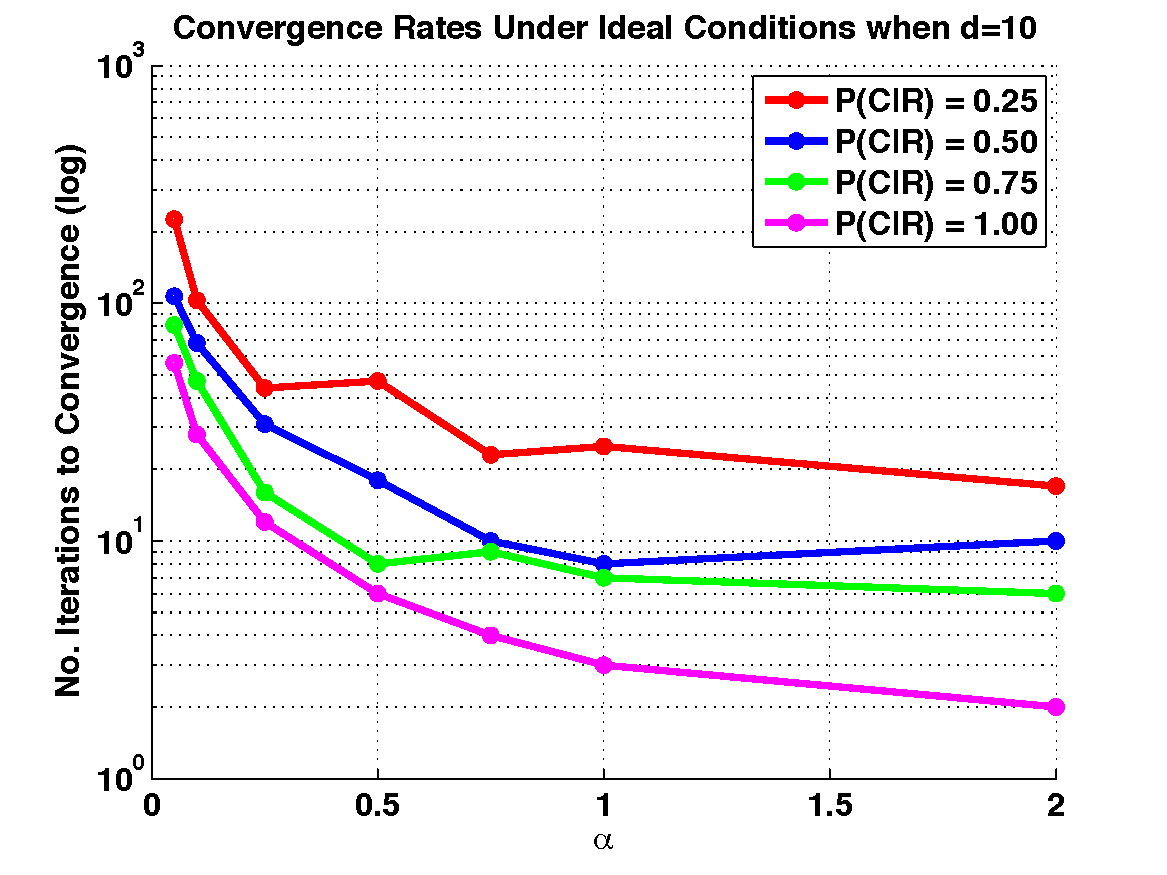
\includegraphics[width=\textwidth]{pics/perfect/simple_multiplicative_d10.pdf}
	  \caption{\textbf{Convergence @ $d=10$}}
	  \label{fig:sub1}
	\end{subfigure}%
	\begin{subfigure}{.33\textwidth}
	  \centering
	  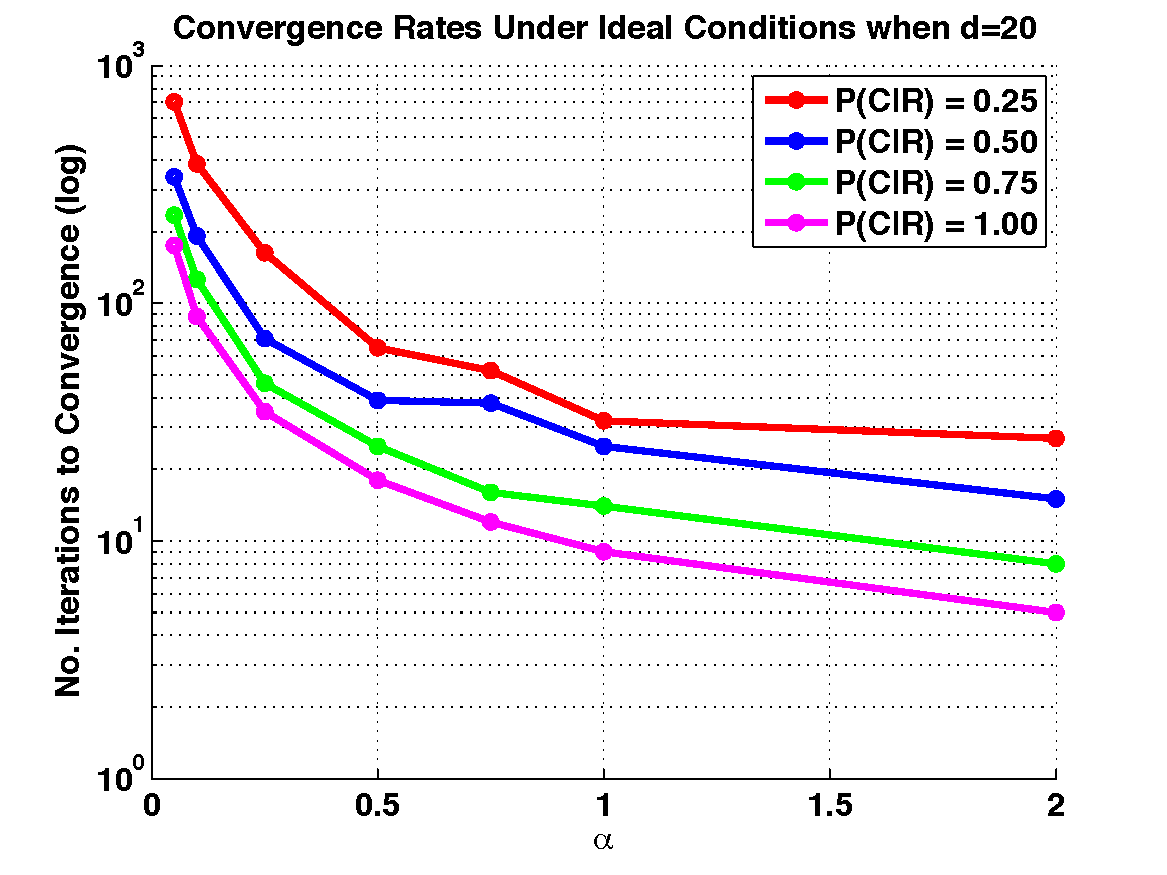
\includegraphics[width=\textwidth]{pics/perfect/simple_multiplicative_d20.pdf}
	  \caption{\textbf{Convergence @ $d=20$}}
	  \label{fig:sub2}
	\end{subfigure}
	\begin{subfigure}{.33\textwidth}
	  \centering
	  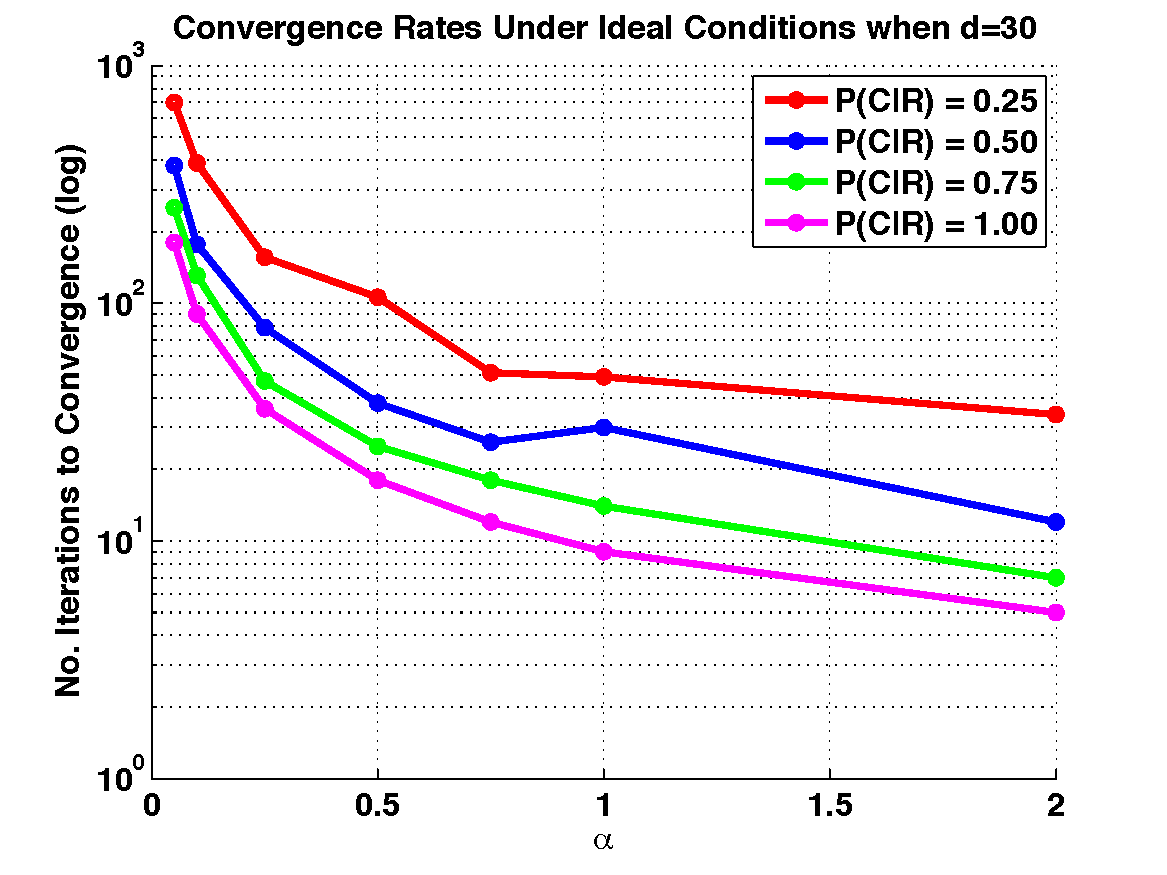
\includegraphics[width=\textwidth]{pics/perfect/simple_multiplicative_d30.pdf}
	  \caption{\textbf{Convergence @ $d=30$}}
	  \label{fig:sub2}
	\end{subfigure}
	
	\caption{\label{fig:perfect_convergence}\textbf{A series of graphs demonstrating the number of iterations required for performance to converge for given $\alpha$ values under ideal conditions. Each graph shows convergence times with varying depth levels.}}
\end{figure*}

Results for models \textbf{PD} and \textbf{PDE} are more complex. For variations of $P(C|R)$ when greater than 0.25, the two models exhibited an unusual behaviour. As the value for $P(C|R)$ was increased, we hypothesised that the number of iterations to reach maximum performance would reduce. Our results showed an almost consistent iteration count for each variation of $P(C|R)$ across the three values of 1.0, 0.75 and 0.5 - as can be seen in Tables \ref{tbl:results_perfect_demotive} and \ref{tbl:results_perfect_view} for models \textbf{PD} and \textbf{PDE} respectively.

\begin{figure}
	\begin{center}
	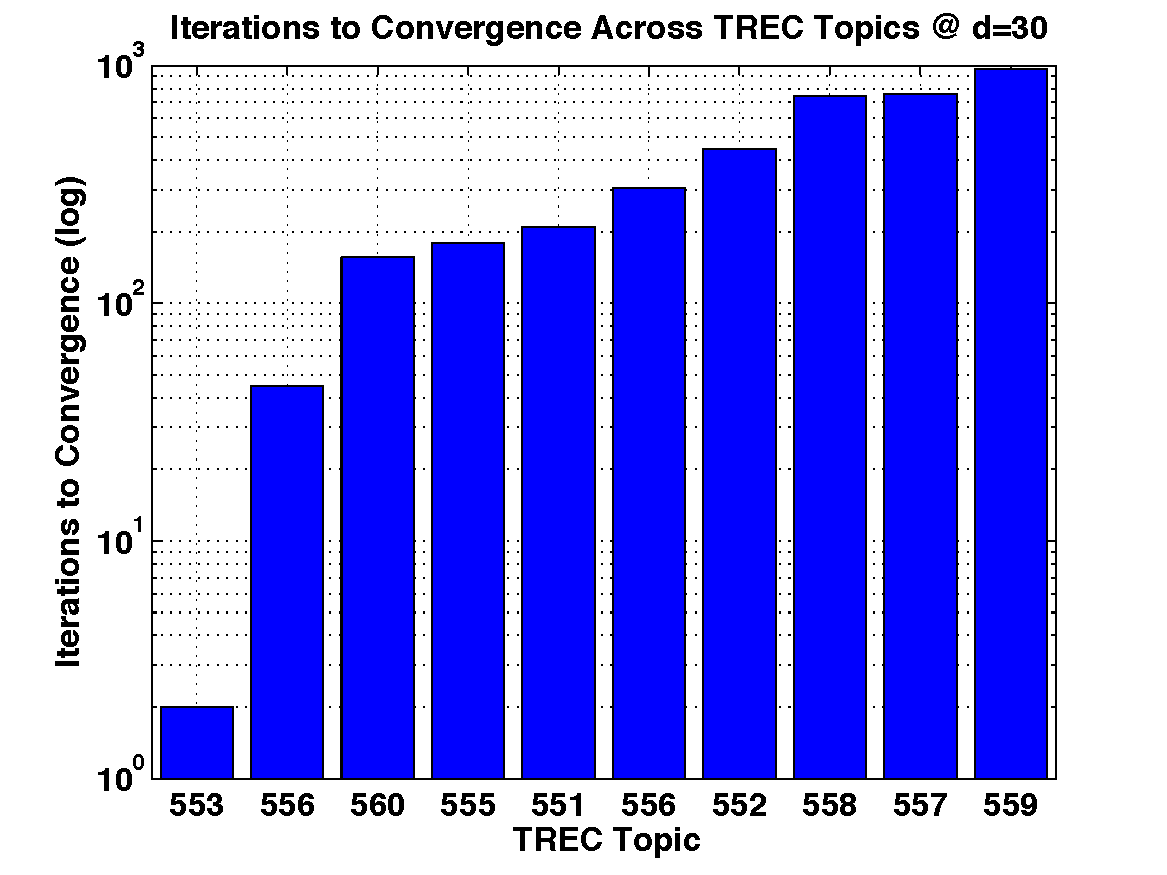
\includegraphics[width=\linewidth]{pics/perfect/perfect_different_topics.pdf}
	\end{center}
	\vspace{-0.5cm}
	\caption{\label{fig:perfect_different_topics}\textbf{A bar chart illustrating the different rates of convergence across TREC topics 551-560 for model \textbf{PD} with $P(C|R) = 0.25$ and $d=30$. Topics are ordered by the iteration count in ascending order.}\vspace{-0.4cm}}
\end{figure}

To examine this behaviour, we ran a further simulation running a sample of queries independently from one another. With model \textbf{PD} and a depth of 10 selected for TREC topics 551-650, we observed that for each query, a different number of iterations were required to reach maximum performance. Such behaviour would explain the consistent iteration count for varying levels of $P(C|R)$. While the performance of some queries may converge early - perhaps due to a potentially limited number of relevant documents high in their baseline rankings - they will almost certainly have to wait for slower queries - with a higher number of relevant documents - to reach maximum performance. With our simulations, as illustrated in Figure \ref{fig:perfect_different_topics}, many of these individual queries took a significant number of iterations to complete.

We also observed that a performance cliff exists for the demotion models, \textbf{PD} and \textbf{PDE}. With a low value of 0.25 set for $P(C|R)$, this meant that a relevant document had a 25\% chance of being clicked during each iteration. As can be seen in Tables \ref{tbl:results_perfect_demotive} and \ref{tbl:results_perfect_view}, such a small probability paired with a high $\beta$ value can have a significant negative impact, with the demotion aspect of each model dominating. Across all three depths for model \textbf{PD} when $P(C|R) = 0.25$ and $\beta = 2.0$, the maximum performance was achieved at the baseline - or 0\textsuperscript{th} iteration. This meant that all further iterations observed a drop in performance.

This finding provides a suggestion to a possible trade-off between the number of iterations that a site administrator would deem acceptable to notice a performance improvement, and the maximum performance he or she can obtain. Such a trade-off could perhaps be influenced by the number of visitors a given website receives, or how willing a particular site's audience would be to look further down results.

\subsection{Including Depth-Proportional Bias}
While clickthrough data are regarded as informative, it has been noted in several studies that such data are inherently biased by the trust they have in the results offered by the search engine used \cite{granka2004eyetracking, joachims2005clickthrough}. Positional bias reduces the probability of a document being examined the further down a ranked results list it appears. For example, a document at rank 1 would have a much higher chance of being examined than a document presented at rank 10.

To incorporate this issue in our study, we performed a series of simulations that examined performance when positional bias was added to clickthrough data. No longer perfect, the probability of examining (and potentially clicking) a document was then set to $1/r$ - or proportional to rank. Including such bias allowed us to address the following overarching question: \emph{what effects does positional bias have on retrieval performance?}

Our depth-proportional simulations were all run with a depth of 30 across all three models as our `perfect' simulations all offered their best performance at this depth. $d=30$ was also considered to be a relatively realistic depth that real-world users of search engines would be willing to look to. Like our `perfect world' simulations, we ran $P(C|R)$ with values of 1.0, 0.75, 0.5 and 0.25. The promotional tuning parameter $\alpha$ was set to a constant 0.75 throughout all simulations. Demotion tuning parameter $\beta$ was varied with the values 0.01, 0.05, 0.10, 0.25, 0.5, 0.75, 1.0 and 2.0 - we did however expect to see best performance from a low $\beta$ value based on our previous findings.

\subsubsection{Results}
To address the operational question posed above, we compared our findings against the results of our `perfect world' simulations. From a simplistic viewpoint, the performance obtained with our depth-proportional is broadly similar to our `perfect world' results. The key difference is however the time taken to reach that maximum performance. A larger number of iterations were required to achieve convergence, as the probability of viewing documents lower down rankings was less than 1.0.

\begin{figure}
	\begin{center}
	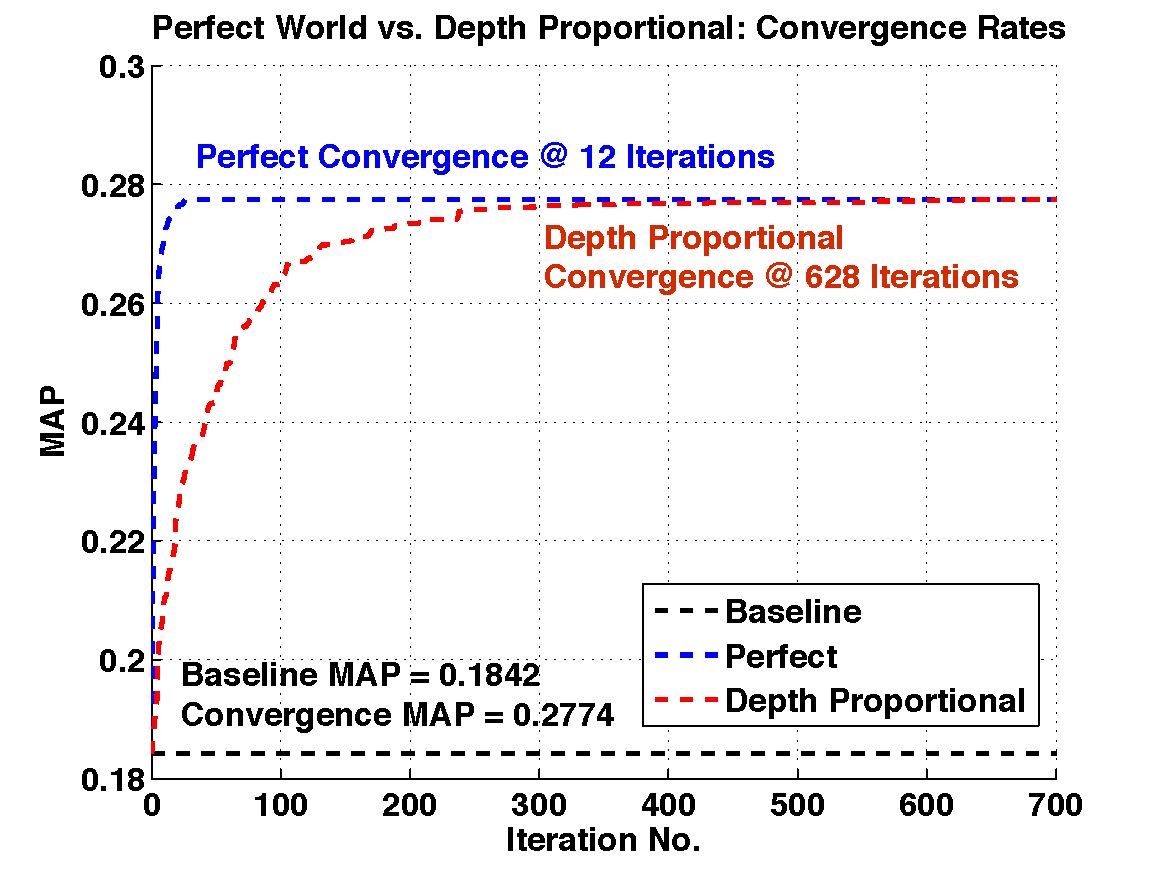
\includegraphics[width=\linewidth]{pics/bias/bias_iterations.pdf}
	\end{center}
	\vspace{-0.5cm}
	\caption{\label{fig:bias_iterations}\textbf{A line graph illustrating the difference in convergence rates for `perfect' and clickthrough data where the probability of viewing and clicking a document is proportional to a given document's depth. Data was generated by the \emph{P} model, where $\alpha = 0.75$, $P(C|R)=0.5$ and $d=30$ for each.}\vspace{-0.5cm}}
\end{figure}

This observation was noted from our promotion-only model \textbf{P}, which showed an identical maximum performance to ideal conditions. Moreover, the number of iterations required for convergence was influenced by the probability of clicking on a relevant document, $P(C|R)$. The higher $P(C|R)$, fewer iterations were required to reach convergence. The iteration count was still much higher than experienced under ideal conditions, as illustrated in Figure \ref{fig:bias_iterations} where ideal and depth-proportional results are compared with $P(C|R) = 0.5$. As the figure demonstrates, a comparable performance was achieved in little over 250 iterations, where MAP was evaluated to be 0.2757. This score was very close to the maximum attainable MAP of 0.2774.

\begin{table*}
	\renewcommand{\arraystretch}{1.3}
	\begin{center}
		\begin{small}
			\begin{tabularx}{\linewidth}{W{2.94cm}|W{1.4cm}|W{1.4cm}|W{1.4cm}|W{1.4cm}|W{1.4cm}|W{1.4cm}|W{1.4cm}|W{1.4cm}W{0.00000001cm}}
				
				& \centering{$\beta=0.01$}
				& \centering{$\beta=0.05$}
				& \centering{$\beta=0.1$}
				& \centering{$\beta=0.25$}
				& \centering{$\beta=0.5$}
				& \centering{$\beta=0.75$}
				& \centering{$\beta=1.0$}
				& \centering{$\beta=2.0$}&
				\tabularnewline[1em]
				\hline
				
				$P(C|R) = 0.0$
				& \multicolumn{8}{c}{\centering{{\tiny\textbf{PD}} 0.1842 ($i = 0$), {\tiny\textbf{PDE}} 0.1842 ($i = 0$)}}&
				\tabularnewline[1.4em]
				\hline
				\hline
				
				\multirow{2}{*}{\vspace{-0.45cm}$P(C|R) = 0.25$}
				& \centering{{\makebox[0pt][c]{{\tiny \textbf{PD}} \textbf{\emph{0.4374}}}\\\makebox[0pt][c]{{\tiny \textbf{PDE}} 0.2776}}}
				& \centering{{\makebox[0pt][c]{{\tiny \textbf{PD}} 0.3022}\\\makebox[0pt][c]{{\tiny \textbf{PDE}} 0.2848}}}
				& \centering{{\makebox[0pt][c]{{\tiny \textbf{PD}} 0.2173}\\\makebox[0pt][c]{{\tiny \textbf{PDE}} \textbf{\emph{0.2921}}}}}
				& \centering{{\makebox[0pt][c]{{\tiny \textbf{PD}} 0.1842}\\\makebox[0pt][c]{{\tiny \textbf{PDE}} 0.2858}}}
				& \centering{{\makebox[0pt][c]{{\tiny \textbf{PD}} 0.1842}\\\makebox[0pt][c]{{\tiny \textbf{PDE}} 0.2515}}}
				& \centering{{\makebox[0pt][c]{{\tiny \textbf{PD}} 0.1842}\\\makebox[0pt][c]{{\tiny \textbf{PDE}} 0.2335}}}
				& \centering{{\makebox[0pt][c]{{\tiny \textbf{PD}} 0.1842}\\\makebox[0pt][c]{{\tiny \textbf{PDE}} 0.2238}}}
				& \centering{{\makebox[0pt][c]{{\tiny \textbf{PD}} 0.1842}\\\makebox[0pt][c]{{\tiny \textbf{PDE}} 0.1842}}}&
				\tabularnewline[1.4em]
				\cline{2-9}
				
				& \centering{{\makebox[0pt][c]{{\tiny \textbf{PD}} $i=988$}\\\makebox[0pt][c]{{\tiny \textbf{PDE}} $i=924$}}}
				& \centering{{\makebox[0pt][c]{{\tiny \textbf{PD}} $i=513$}\\\makebox[0pt][c]{{\tiny \textbf{PDE}} $i=1000$}}}
				& \centering{{\makebox[0pt][c]{{\tiny \textbf{PD}} $i=88$}\\\makebox[0pt][c]{{\tiny \textbf{PDE}} $i=1000$}}}
				& \centering{{\makebox[0pt][c]{{\tiny \textbf{PD}} $i=0$}\\\makebox[0pt][c]{{\tiny \textbf{PDE}} $i=969$}}}
				& \centering{{\makebox[0pt][c]{{\tiny \textbf{PD}} $i=0$}\\\makebox[0pt][c]{{\tiny \textbf{PDE}} $i=890$}}}
				& \centering{{\makebox[0pt][c]{{\tiny \textbf{PD}} $i=0$}\\\makebox[0pt][c]{{\tiny \textbf{PDE}} $i=1000$}}}
				& \centering{{\makebox[0pt][c]{{\tiny \textbf{PD}} $i=0$}\\\makebox[0pt][c]{{\tiny \textbf{PDE}} $i=1000$}}}
				& \centering{{\makebox[0pt][c]{{\tiny \textbf{PD}} $i=0$}\\\makebox[0pt][c]{{\tiny \textbf{PDE}} $i=0$}}}&
				\tabularnewline[1.4em]
				\hline
				\hline
				
				\multirow{2}{*}{\vspace{-0.45cm}$P(C|R) = 0.5$}
				& \centering{{\makebox[0pt][c]{{\tiny \textbf{PD}} \textbf{\emph{0.4767}}}\\\makebox[0pt][c]{{\tiny \textbf{PDE}} 0.2776}}}
				& \centering{{\makebox[0pt][c]{{\tiny \textbf{PD}} 0.4263}\\\makebox[0pt][c]{{\tiny \textbf{PDE}} 0.2847}}}
				& \centering{{\makebox[0pt][c]{{\tiny \textbf{PD}} 0.3208}\\\makebox[0pt][c]{{\tiny \textbf{PDE}} 0.2881}}}
				& \centering{{\makebox[0pt][c]{{\tiny \textbf{PD}} 0.2139}\\\makebox[0pt][c]{{\tiny \textbf{PDE}} 0.3084}}}
				& \centering{{\makebox[0pt][c]{{\tiny \textbf{PD}} 0.1842}\\\makebox[0pt][c]{{\tiny \textbf{PDE}} \textbf{\emph{0.3226}}}}}
				& \centering{{\makebox[0pt][c]{{\tiny \textbf{PD}} 0.1842}\\\makebox[0pt][c]{{\tiny \textbf{PDE}} 0.3049}}}
				& \centering{{\makebox[0pt][c]{{\tiny \textbf{PD}} 0.1842}\\\makebox[0pt][c]{{\tiny \textbf{PDE}} 0.2614}}}
				& \centering{{\makebox[0pt][c]{{\tiny \textbf{PD}} 0.1842}\\\makebox[0pt][c]{{\tiny \textbf{PDE}} 0.2618}}}&
				\tabularnewline[1.4em]
				\cline{2-9}
				
				& \centering{{\makebox[0pt][c]{{\tiny \textbf{PD}} $i=1000$}\\\makebox[0pt][c]{{\tiny \textbf{PDE}} $i=501$}}}
				& \centering{{\makebox[0pt][c]{{\tiny \textbf{PD}} $i=1000$}\\\makebox[0pt][c]{{\tiny \textbf{PDE}} $i=812$}}}
				& \centering{{\makebox[0pt][c]{{\tiny \textbf{PD}} $i=211$}\\\makebox[0pt][c]{{\tiny \textbf{PDE}} $i=1000$}}}
				& \centering{{\makebox[0pt][c]{{\tiny \textbf{PD}} $i=23$}\\\makebox[0pt][c]{{\tiny \textbf{PDE}} $i=1000$}}}
				& \centering{{\makebox[0pt][c]{{\tiny \textbf{PD}} $i=0$}\\\makebox[0pt][c]{{\tiny \textbf{PDE}} $i=1000$}}}
				& \centering{{\makebox[0pt][c]{{\tiny \textbf{PD}} $i=0$}\\\makebox[0pt][c]{{\tiny \textbf{PDE}} $i=1000$}}}
				& \centering{{\makebox[0pt][c]{{\tiny \textbf{PD}} $i=0$}\\\makebox[0pt][c]{{\tiny \textbf{PDE}} $i=305$}}}
				& \centering{{\makebox[0pt][c]{{\tiny \textbf{PD}} $i=0$}\\\makebox[0pt][c]{{\tiny \textbf{PDE}} $i=977$}}}&
				\tabularnewline[1.4em]
				\hline
				\hline
				
				\multirow{2}{*}{\vspace{-0.45cm}$P(C|R) = 0.75$}
				& \centering{{\makebox[0pt][c]{{\tiny \textbf{PD}} 0.4938}\\\makebox[0pt][c]{{\tiny \textbf{PDE}} 0.2776}}}
				& \centering{{\makebox[0pt][c]{{\tiny \textbf{PD}} \textbf{\emph{0.4985}}}\\\makebox[0pt][c]{{\tiny \textbf{PDE}} 0.281}}}
				& \centering{{\makebox[0pt][c]{{\tiny \textbf{PD}} 0.3852}\\\makebox[0pt][c]{{\tiny \textbf{PDE}} 0.2884}}}
				& \centering{{\makebox[0pt][c]{{\tiny \textbf{PD}} 0.2569}\\\makebox[0pt][c]{{\tiny \textbf{PDE}} 0.3076}}}
				& \centering{{\makebox[0pt][c]{{\tiny \textbf{PD}} 0.2072}\\\makebox[0pt][c]{{\tiny \textbf{PDE}} 0.3257}}}
				& \centering{{\makebox[0pt][c]{{\tiny \textbf{PD}} 0.1939}\\\makebox[0pt][c]{{\tiny \textbf{PDE}} 0.3323}}}
				& \centering{{\makebox[0pt][c]{{\tiny \textbf{PD}} 0.1842}\\\makebox[0pt][c]{{\tiny \textbf{PDE}} 0.3355}}}
				& \centering{{\makebox[0pt][c]{{\tiny \textbf{PD}} 0.1842}\\\makebox[0pt][c]{{\tiny \textbf{PDE}} \emph{\textbf{0.3377}}}}}&
				\tabularnewline[1.4em]
				\cline{2-9}
				
				& \centering{{\makebox[0pt][c]{{\tiny \textbf{PD}} $i=1000$}\\\makebox[0pt][c]{{\tiny \textbf{PDE}} $i=350$}}}
				& \centering{{\makebox[0pt][c]{{\tiny \textbf{PD}} $i=981$}\\\makebox[0pt][c]{{\tiny \textbf{PDE}} $i=314$}}}
				& \centering{{\makebox[0pt][c]{{\tiny \textbf{PD}} $i=413$}\\\makebox[0pt][c]{{\tiny \textbf{PDE}} $i=951$}}}
				& \centering{{\makebox[0pt][c]{{\tiny \textbf{PD}} $i=143$}\\\makebox[0pt][c]{{\tiny \textbf{PDE}} $i=974$}}}
				& \centering{{\makebox[0pt][c]{{\tiny \textbf{PD}} $i=18$}\\\makebox[0pt][c]{{\tiny \textbf{PDE}} $i=1000$}}}
				& \centering{{\makebox[0pt][c]{{\tiny \textbf{PD}} $i=8$}\\\makebox[0pt][c]{{\tiny \textbf{PDE}} $i=1000$}}}
				& \centering{{\makebox[0pt][c]{{\tiny \textbf{PD}} $i=0$}\\\makebox[0pt][c]{{\tiny \textbf{PDE}} $i=1000$}}}
				& \centering{{\makebox[0pt][c]{{\tiny \textbf{PD}} $i=0$}\\\makebox[0pt][c]{{\tiny \textbf{PDE}} $i=1000$}}}&
				\tabularnewline[1.4em]
				\hline
				\hline
				
				\multirow{2}{*}{\vspace{-0.45cm}$P(C|R) = 1.0$}
				& \centering{{\makebox[0pt][c]{{\tiny \textbf{PD}} 0.4998}\\\makebox[0pt][c]{{\tiny \textbf{PDE}} 0.2774}}}
				& \centering{{\makebox[0pt][c]{{\tiny \textbf{PD}} \textbf{0.5417}}\\\makebox[0pt][c]{{\tiny \textbf{PDE}} 0.2847}}}
				& \centering{{\makebox[0pt][c]{{\tiny \textbf{PD}} 0.4464}\\\makebox[0pt][c]{{\tiny \textbf{PDE}} 0.2894}}}
				& \centering{{\makebox[0pt][c]{{\tiny \textbf{PD}} 0.2868}\\\makebox[0pt][c]{{\tiny \textbf{PDE}} 0.3088}}}
				& \centering{{\makebox[0pt][c]{{\tiny \textbf{PD}} 0.2169}\\\makebox[0pt][c]{{\tiny \textbf{PDE}} 0.3261}}}
				& \centering{{\makebox[0pt][c]{{\tiny \textbf{PD}} 0.2171}\\\makebox[0pt][c]{{\tiny \textbf{PDE}} 0.3319}}}
				& \centering{{\makebox[0pt][c]{{\tiny \textbf{PD}} 0.1842}\\\makebox[0pt][c]{{\tiny \textbf{PDE}} 0.3379}}}
				& \centering{{\makebox[0pt][c]{{\tiny \textbf{PD}} 0.1842}\\\makebox[0pt][c]{{\tiny \textbf{PDE}} \textbf{0.3489}}}}&
				\tabularnewline[1.4em]
				\cline{2-9}
				
				& \centering{{\makebox[0pt][c]{{\tiny \textbf{PD}} $i=1000$}\\\makebox[0pt][c]{{\tiny \textbf{PDE}} $i=277$}}}
				& \centering{{\makebox[0pt][c]{{\tiny \textbf{PD}} $i=978$}\\\makebox[0pt][c]{{\tiny \textbf{PDE}} $i=819$}}}
				& \centering{{\makebox[0pt][c]{{\tiny \textbf{PD}} $i=979$}\\\makebox[0pt][c]{{\tiny \textbf{PDE}} $i=1000$}}}
				& \centering{{\makebox[0pt][c]{{\tiny \textbf{PD}} $i=173$}\\\makebox[0pt][c]{{\tiny \textbf{PDE}} $i=1000$}}}
				& \centering{{\makebox[0pt][c]{{\tiny \textbf{PD}} $i=27$}\\\makebox[0pt][c]{{\tiny \textbf{PDE}} $i=1000$}}}
				& \centering{{\makebox[0pt][c]{{\tiny \textbf{PD}} $i=16$}\\\makebox[0pt][c]{{\tiny \textbf{PDE}} $i=1000$}}}
				& \centering{{\makebox[0pt][c]{{\tiny \textbf{PD}} $i=0$}\\\makebox[0pt][c]{{\tiny \textbf{PDE}} $i=1000$}}}
				& \centering{{\makebox[0pt][c]{{\tiny \textbf{PD}} $i=0$}\\\makebox[0pt][c]{{\tiny \textbf{PDE}} $i=1000$}}}&
				\tabularnewline[1.4em]
				
			\end{tabularx}
		\end{small}
	\end{center}

	\vspace{-0.4cm}
	\caption{\textbf{Table highlighting the best MAP values obtained and corresponding simulation counts for models \emph{PD} and \emph{PDE} with depth-proportional clickthrough data. $P(C|R)$ is varied, and both $d=30$ and $\alpha=0.75$ are constant.}}
	\label{tbl:results_biased_demotion}
\end{table*}

Despite these intuitive findings, interesting observations were made with the two promotion/demotion models, \textbf{PD} and \textbf{PDE}. For \textbf{PD}, it was observed that performance was at its highest when $\beta$ was set to a low value. When $P(C|R)$ was also set to a low value of 0.25, a MAP of 0.4374 was obtained when $\beta = 0.01$. This value is higher than the MAP of 0.3022 observed for $\beta = 0.05$. However, with $P(C|R)$ set to 1.0, the best performance of 0.5417 was attained with $\beta = 0.05$.

This finding suggests that there is a possible relationship between the probability of clicks on a relevant document, $P(C|R)$, and the weighting applied to the demotion aspect of clickthrough models, $\beta$. If for example users of a website search engine were to click on more and more relevant documents, the demotion weighting can be \emph{slightly} increased due to the increased confidence in users' clicks signifying relevance to a query. The greater weighting for demotion would therefore allow documents that are considered irrelevant to be demoted down rankings more quickly, yielding a greater performance gain. Care must be taken regarding the choice of $\beta$ value - as seen in Table \ref{tbl:results_biased_demotion}, a $\beta$ value greater than 0.05 gave steadily reduced performance - dropping below baseline values for high $\beta$ values.

Also shown in Table \ref{tbl:results_biased_demotion} are our results for \textbf{PDE}. Compared to \textbf{PD}, we found significant differences in the way the model reacted to differing parameter variations. As expected, better performance was observed as $P(C|R)$ increased. However, as $\beta$ increased, so did performance - even past the \textbf{PD} threshold of 0.05. Indeed, the highest MAP of 0.3489 for \textbf{PDE} was observed when $P(C|R) = 1.0$ and $\beta = 2.0$. Such behaviour could be attributed to the greater demoting power \textbf{PDE} had as $\beta$ increased. Examining the definition of the model in Equation \ref{eqn:pde}, the greater the chance the demotion aspect of the model would dominate the promotion aspect as $\beta$ was set to a higher value. Increasing $\beta$ therefore attempted to mitigate the effect of introducing depth-proportional bias.

\subsection{Varying Noise}
One of the major disadvantages of clickthrough data are its tendency of being susceptible to noise. Noise - where users click on documents that are irrelevant to a query - cannot be avoided in a real-world environment. Thus, any models developed that utilise clickthrough data must have a degree of tolerance to noise - which inevitably comes with the sacrifice of performance. This therefore leads us to ask the operational question: \emph{how does including noise in clickthrough data affect performance?}

To address this question, we conducted a further series of simulations. Coupled with positional bias, we began to vary the probability of a click on irrelevant documents, $P(C|N)$, along with $P(C|R)$. Up until this point, all simulations had been run free of noise, with $P(C|N) = 0.0$. With these simulations, we also set the probability of examining a document to be proportional to depth, and like previous simulations, set $\alpha = 0.75$. For our promotion/demotion models, $\beta$ was fixed at 0.05 due to the positive outcomes the value had with previous simulations. However, findings of our depth-proportional simulations pushed us towards running further simulations for models \textbf{PD} and \textbf{PDE} where $\beta$ was set to 0.10, 0.25 and 2.0. These simulations were then repeated without positional bias, allowing us to make a direct comparison with our `perfect world' simulations.

\subsubsection{Results}\label{sec:results:noise}
Results from our simulations incorporating noise show that performance is affected - in terms of the maximum that can be attained, and the length of time required to reach it. Previous simulations have demonstrated that the behaviour of model \textbf{P} has been straightforward to follow. We therefore use the results from \textbf{P} to explain basic behavioural changes with clickthrough data as noise is varied.

Table \ref{tbl:noisy_multiplicative} shows the highest MAP figures obtained for varying levels of $P(C|R)$ and $P(C|N)$ across clickthrough simulations incorporating noise, and noise with depth-proportional viewing. The table also shows the number of iterations that were required to reach the performance highs.

\begin{figure}[t!]
	\begin{center}
	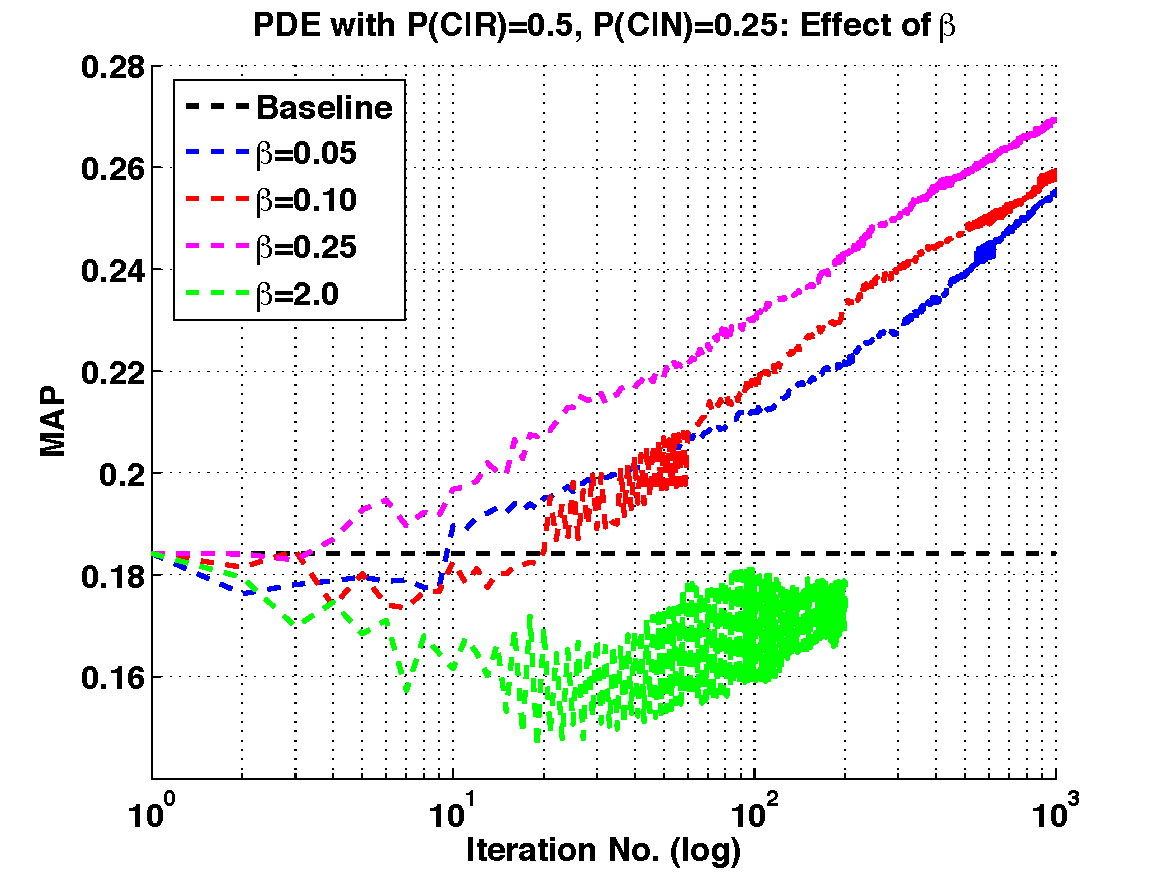
\includegraphics[width=\linewidth]{pics/noise/noise_pde_beta.pdf}
	\end{center}
	\vspace{-0.5cm}
	\caption{\label{fig:noise_pde_beta}\textbf{A line graph illustrating performance vs. iterations with different $\beta$ values for \emph{PDE} using noisy data and depth-proportional views. Here, $P(C|R) = 0.5$ and $P(C|N) = 0.25$.}\vspace{-0.25cm}}
\end{figure}

Our results show that as $P(C|R)$ increases, performance also increases. However, as we begin to introduce noise by increasing the value of $P(C|N)$, we observe two key behaviours which are exerted:

\begin{enumerate}
	
	\item{convergence to maximum performance takes significantly longer; or}
	
	\item{no performance improvement is observed whatsoever.}
	
\end{enumerate}

To provide an example of the former observation, we can see from Table \ref{tbl:noisy_multiplicative} that when $P(C|R) = 0.5$ and $P(C|N) = 0.25$, performance for our noise-only simulation converged at the highest attainable MAP of 0.2774 after 82 iterations. This is in comparison to the 12 iterations that our simulations run ideal conditions took (see Table \ref{tbl:results_perfect_demotive}). We also observed that including positional bias in our simulations increases the number of iterations required for convergence to 992 (with a cap at 1000) - and would require even more to reach the maximum attainable MAP of 0.2774.

Results also show a significant drop in performance as noise is introduced. This can be partly explained by the na\"{i}vety of \textbf{P}, detailed in Section \ref{sec:method:models:promo}. As $P(C|N)$ is increased, more irrelevant documents are clicked and promoted. As \textbf{P} assumes clicks signify relevance, tolerances for noise with the model are therefore low.

\begin{table}[t!]
	\renewcommand{\arraystretch}{1.3}
	\begin{center}
		\begin{small}
			\begin{tabularx}{\linewidth}{W{1.29cm}|W{1.29cm}|W{1.29cm}|W{1.29cm}|W{1.29cm}W{0.00000001cm}}
				
			 	& \centering{{\makebox[0pt][c]{$PN = 0.25$}}} & \centering{$PN = 0.5$} & \centering{{\makebox[0pt][c]{$PN = 0.75$}}} & \centering{$PN = 1.0$}&
				\tabularnewline[1.4em]
				\hline
				
				\multirow{2}{*}{\vspace{-0.45cm}$PR = 0.25$}
				& \centering{{\makebox[0pt][c]{{\tiny \textbf{ND}} 0.1842}\\\makebox[0pt][c]{{\tiny \textbf{N}} 0.1842}}}
				& \centering{{\makebox[0pt][c]{{\tiny \textbf{ND}} 0.1842}\\\makebox[0pt][c]{{\tiny \textbf{N}} 0.1842}}}
				& \centering{{\makebox[0pt][c]{{\tiny \textbf{ND}} 0.1842}\\\makebox[0pt][c]{{\tiny \textbf{N}} 0.1842}}}
				& \centering{{\makebox[0pt][c]{{\tiny \textbf{ND}} 0.1842}\\\makebox[0pt][c]{{\tiny \textbf{N}} 0.1842}}}&
				\tabularnewline[1.4em]
				\cline{2-5}
				
				& \centering{{\makebox[0pt][c]{{\tiny \textbf{ND}} $i=0$}\\\makebox[0pt][c]{{\tiny \textbf{N}} $i=0$}}}
				& \centering{{\makebox[0pt][c]{{\tiny \textbf{ND}} $i=0$}\\\makebox[0pt][c]{{\tiny \textbf{N}} $i=0$}}}
				& \centering{{\makebox[0pt][c]{{\tiny \textbf{ND}} $i=0$}\\\makebox[0pt][c]{{\tiny \textbf{N}} $i=0$}}}
				& \centering{{\makebox[0pt][c]{{\tiny \textbf{ND}} $i=0$}\\\makebox[0pt][c]{{\tiny \textbf{N}} $i=0$}}}&
				\tabularnewline[1.4em]
				\hline
				
				\multirow{2}{*}{\vspace{-0.45cm}$PR = 0.5$}
				& \centering{{\makebox[0pt][c]{{\tiny \textbf{ND}} \textbf{0.2527}}\\\makebox[0pt][c]{{\tiny \textbf{N}} \textbf{0.2774}}}}
				& \centering{{\makebox[0pt][c]{{\tiny \textbf{ND}} 0.1842}\\\makebox[0pt][c]{{\tiny \textbf{N}} 0.1842}}}
				& \centering{{\makebox[0pt][c]{{\tiny \textbf{ND}} 0.1842}\\\makebox[0pt][c]{{\tiny \textbf{N}} 0.1842}}}
				& \centering{{\makebox[0pt][c]{{\tiny \textbf{ND}} 0.1842}\\\makebox[0pt][c]{{\tiny \textbf{N}} 0.1842}}}&
				\tabularnewline[1.4em]
				\cline{2-5}
				
				& \centering{{\makebox[0pt][c]{{\tiny \textbf{ND}} $i=992$}\\\makebox[0pt][c]{{\tiny \textbf{N}} $i=82$}}}
				& \centering{{\makebox[0pt][c]{{\tiny \textbf{ND}} $i=0$}\\\makebox[0pt][c]{{\tiny \textbf{N}} $i=0$}}}
				& \centering{{\makebox[0pt][c]{{\tiny \textbf{ND}} $i=0$}\\\makebox[0pt][c]{{\tiny \textbf{N}} $i=0$}}}
				& \centering{{\makebox[0pt][c]{{\tiny \textbf{ND}} $i=0$}\\\makebox[0pt][c]{{\tiny \textbf{N}} $i=0$}}}&
				\tabularnewline[1.4em]
				\hline
				
				\multirow{2}{*}{\vspace{-0.45cm}$PR = 0.75$}
				& \centering{{\makebox[0pt][c]{{\tiny \textbf{ND}} \textbf{0.2769}}\\\makebox[0pt][c]{{\tiny \textbf{N}} \textbf{0.2774}}}}
				& \centering{{\makebox[0pt][c]{{\tiny \textbf{ND}} \textbf{0.2291}}\\\makebox[0pt][c]{{\tiny \textbf{N}} \textbf{0.2774}}}}
				& \centering{{\makebox[0pt][c]{{\tiny \textbf{ND}} \textbf{0.1884}}\\\makebox[0pt][c]{{\tiny \textbf{N}} 0.1842}}}
				& \centering{{\makebox[0pt][c]{{\tiny \textbf{ND}} 0.1842}\\\makebox[0pt][c]{{\tiny \textbf{N}} 0.1842}}}&
				\tabularnewline[1.4em]
				\cline{2-5}
				
				& \centering{{\makebox[0pt][c]{{\tiny \textbf{ND}} $i=947$}\\\makebox[0pt][c]{{\tiny \textbf{N}} $i=39$}}}
				& \centering{{\makebox[0pt][c]{{\tiny \textbf{ND}} $i=997$}\\\makebox[0pt][c]{{\tiny \textbf{N}} $i=95$}}}
				& \centering{{\makebox[0pt][c]{{\tiny \textbf{ND}} $i=1$}\\\makebox[0pt][c]{{\tiny \textbf{N}} $i=0$}}}
				& \centering{{\makebox[0pt][c]{{\tiny \textbf{ND}} $i=0$}\\\makebox[0pt][c]{{\tiny \textbf{N}} $i=0$}}}&
				\tabularnewline[1.4em]
				\hline
				
				\multirow{2}{*}{\vspace{-0.45cm}$PR = 1.0$}
				& \centering{{\makebox[0pt][c]{{\tiny \textbf{ND}} \textbf{0.2774}}\\\makebox[0pt][c]{{\tiny \textbf{N}} \textbf{0.2774}}}}
				& \centering{{\makebox[0pt][c]{{\tiny \textbf{ND}} \textbf{0.2625}}\\\makebox[0pt][c]{{\tiny \textbf{N}} \textbf{0.2774}}}}
				& \centering{{\makebox[0pt][c]{{\tiny \textbf{ND}} \textbf{0.2176}}\\\makebox[0pt][c]{{\tiny \textbf{N}} \textbf{0.2774}}}}
				& \centering{{\makebox[0pt][c]{{\tiny \textbf{ND}} \textbf{0.1845}}\\\makebox[0pt][c]{{\tiny \textbf{N}} 0.1842}}}&
				\tabularnewline[1.4em]
				\cline{2-5}
				
				& \centering{{\makebox[0pt][c]{{\tiny \textbf{ND}} $i=713$}\\\makebox[0pt][c]{{\tiny \textbf{N}} $i=16$}}}
				& \centering{{\makebox[0pt][c]{{\tiny \textbf{ND}} $i=999$}\\\makebox[0pt][c]{{\tiny \textbf{N}} $i=29$}}}
				& \centering{{\makebox[0pt][c]{{\tiny \textbf{ND}} $i=983$}\\\makebox[0pt][c]{{\tiny \textbf{N}} $i=66$}}}
				& \centering{{\makebox[0pt][c]{{\tiny \textbf{ND}} $i=2$}\\\makebox[0pt][c]{{\tiny \textbf{N}} $i=0$}}}&
				\tabularnewline[1.4em]
				
			\end{tabularx}
		\end{small}
	\end{center}
	
	\vspace{-0.4cm}
	\caption{\textbf{Table illustrating the highest MAP values obtained and associated iteration counts for model \emph{P}, with variations in the probabilities for relevant and irrelevant clicks. Data in the table is for noise and depth-proportional \emph{(ND)}, and noise only \emph{(N)}. For brevity, \emph{PR} in this table signifies $P(C|R)$, and \emph{PN} signifies $P(C|N)$. The baseline MAP was 0.1842, and the maximum attainable MAP at $d=30$ was 0.2774.}\vspace{-0.4cm}}
	\label{tbl:noisy_multiplicative}
\end{table}

Results from our promotion/demotion models \textbf{PD} and \textbf{PDE} followed a similar trend to those of \textbf{P}. Although a similar performance `cliff' existed whereafter no improvements were made, we did observe notable increases over \textbf{P} before the `cliff' was reached. Performance also dropped at a much slower rate, suggesting that \textbf{PD} and \textbf{PDE} were much more tolerable to noise. Tables \hyperref[tbl:noisy_pd]{7} and \hyperref[tbl:noisy_pde]{8} present the highest attained MAP values and respective iteration counts for models \textbf{PD} and \textbf{PDE} respectively.

\begin{table*}

	\begin{subtable}{\columnwidth}
			\begin{small}
				\begin{tabularx}{\linewidth}{W{1.29cm}|W{1.29cm}|W{1.29cm}|W{1.29cm}|W{1.29cm}W{0.00000001cm}}

				 	\centering{{\makebox[0pt][c]{{\tiny \textbf{ND}} $\beta = 0.05$}\\\makebox[0pt][c]{{\tiny \textbf{N}} $\beta = 2.0$}}}
					& \centering{{\makebox[0pt][c]{$PN = 0.25$}}} & \centering{$PN = 0.5$} & \centering{{\makebox[0pt][c]{$PN = 0.75$}}} & \centering{$PN = 1.0$}&
					\tabularnewline[1.4em]
					\hline

					\multirow{2}{*}{\vspace{-0.45cm}$PR = 0.25$}
					& \centering{{\makebox[0pt][c]{{\tiny \textbf{ND}} 0.1842}\\\makebox[0pt][c]{{\tiny \textbf{N}} 0.1842}}}
					& \centering{{\makebox[0pt][c]{{\tiny \textbf{ND}} 0.1842}\\\makebox[0pt][c]{{\tiny \textbf{N}} 0.1842}}}
					& \centering{{\makebox[0pt][c]{{\tiny \textbf{ND}} 0.1842}\\\makebox[0pt][c]{{\tiny \textbf{N}} 0.1842}}}
					& \centering{{\makebox[0pt][c]{{\tiny \textbf{ND}} 0.1842}\\\makebox[0pt][c]{{\tiny \textbf{N}} 0.1842}}}&
					\tabularnewline[1.4em]
					\cline{2-5}

					& \centering{{\makebox[0pt][c]{{\tiny \textbf{ND}} $i=0$}\\\makebox[0pt][c]{{\tiny \textbf{N}} $i=0$}}}
					& \centering{{\makebox[0pt][c]{{\tiny \textbf{ND}} $i=0$}\\\makebox[0pt][c]{{\tiny \textbf{N}} $i=0$}}}
					& \centering{{\makebox[0pt][c]{{\tiny \textbf{ND}} $i=0$}\\\makebox[0pt][c]{{\tiny \textbf{N}} $i=0$}}}
					& \centering{{\makebox[0pt][c]{{\tiny \textbf{ND}} $i=0$}\\\makebox[0pt][c]{{\tiny \textbf{N}} $i=0$}}}&
					\tabularnewline[1.4em]
					\hline

					\multirow{2}{*}{\vspace{-0.45cm}$PR = 0.5$}
					& \centering{{\makebox[0pt][c]{{\tiny \textbf{ND}} \textbf{0.2350}}\\\makebox[0pt][c]{{\tiny \textbf{N}} 0.1842}}}
					& \centering{{\makebox[0pt][c]{{\tiny \textbf{ND}} 0.1842}\\\makebox[0pt][c]{{\tiny \textbf{N}} 0.1842}}}
					& \centering{{\makebox[0pt][c]{{\tiny \textbf{ND}} 0.1842}\\\makebox[0pt][c]{{\tiny \textbf{N}} 0.1842}}}
					& \centering{{\makebox[0pt][c]{{\tiny \textbf{ND}} 0.1842}\\\makebox[0pt][c]{{\tiny \textbf{N}} 0.1842}}}&
					\tabularnewline[1.4em]
					\cline{2-5}

					& \centering{{\makebox[0pt][c]{{\tiny \textbf{ND}} $i=416$}\\\makebox[0pt][c]{{\tiny \textbf{N}} $i=0$}}}
					& \centering{{\makebox[0pt][c]{{\tiny \textbf{ND}} $i=0$}\\\makebox[0pt][c]{{\tiny \textbf{N}} $i=0$}}}
					& \centering{{\makebox[0pt][c]{{\tiny \textbf{ND}} $i=0$}\\\makebox[0pt][c]{{\tiny \textbf{N}} $i=0$}}}
					& \centering{{\makebox[0pt][c]{{\tiny \textbf{ND}} $i=0$}\\\makebox[0pt][c]{{\tiny \textbf{N}} $i=0$}}}&
					\tabularnewline[1.4em]
					\hline

					\multirow{2}{*}{\vspace{-0.45cm}$PR = 0.75$}
					& \centering{{\makebox[0pt][c]{{\tiny \textbf{ND}} \textbf{0.4000}}\\\makebox[0pt][c]{{\tiny \textbf{N}} \textbf{0.6132}}}}
					& \centering{{\makebox[0pt][c]{{\tiny \textbf{ND}} \textbf{0.2102}}\\\makebox[0pt][c]{{\tiny \textbf{N}} \textbf{0.5472}}}}
					& \centering{{\makebox[0pt][c]{{\tiny \textbf{ND}} 0.1842}\\\makebox[0pt][c]{{\tiny \textbf{N}} 0.1842}}}
					& \centering{{\makebox[0pt][c]{{\tiny \textbf{ND}} 0.1842}\\\makebox[0pt][c]{{\tiny \textbf{N}} 0.1842}}}&
					\tabularnewline[1.4em]
					\cline{2-5}

					& \centering{{\makebox[0pt][c]{{\tiny \textbf{ND}} $i=978$}\\\makebox[0pt][c]{{\tiny \textbf{N}} $i=915$}}}
					& \centering{{\makebox[0pt][c]{{\tiny \textbf{ND}} $i=760$}\\\makebox[0pt][c]{{\tiny \textbf{N}} $i=984$}}}
					& \centering{{\makebox[0pt][c]{{\tiny \textbf{ND}} $i=0$}\\\makebox[0pt][c]{{\tiny \textbf{N}} $i=0$}}}
					& \centering{{\makebox[0pt][c]{{\tiny \textbf{ND}} $i=0$}\\\makebox[0pt][c]{{\tiny \textbf{N}} $i=0$}}}&
					\tabularnewline[1.4em]
					\hline

					\multirow{2}{*}{\vspace{-0.45cm}$PR = 1.0$}
					& \centering{{\makebox[0pt][c]{{\tiny \textbf{ND}} \textbf{0.467}}\\\makebox[0pt][c]{{\tiny \textbf{N}} \textbf{0.6724}}}}
					& \centering{{\makebox[0pt][c]{{\tiny \textbf{ND}} \textbf{0.3241}}\\\makebox[0pt][c]{{\tiny \textbf{N}} \textbf{0.6719}}}}
					& \centering{{\makebox[0pt][c]{{\tiny \textbf{ND}} \textbf{0.2045}}\\\makebox[0pt][c]{{\tiny \textbf{N}} \textbf{0.4586}}}}
					& \centering{{\makebox[0pt][c]{{\tiny \textbf{ND}} 0.1842}\\\makebox[0pt][c]{{\tiny \textbf{N}} 0.1842}}}&
					\tabularnewline[1.4em]
					\cline{2-5}

					& \centering{{\makebox[0pt][c]{{\tiny \textbf{ND}} $i=994$}\\\makebox[0pt][c]{{\tiny \textbf{N}} $i=447$}}}
					& \centering{{\makebox[0pt][c]{{\tiny \textbf{ND}} $i=1000$}\\\makebox[0pt][c]{{\tiny \textbf{N}} $i=939$}}}
					& \centering{{\makebox[0pt][c]{{\tiny \textbf{ND}} $i=529$}\\\makebox[0pt][c]{{\tiny \textbf{N}} $i=997$}}}
					& \centering{{\makebox[0pt][c]{{\tiny \textbf{ND}} $i=0$}\\\makebox[0pt][c]{{\tiny \textbf{N}} $i=0$}}}&
					\tabularnewline[1.4em]

				\end{tabularx}
			\end{small}

		\caption*{\textbf{Table 7: PD}}
		\label{tbl:noisy_pd}

	\end{subtable}
	\hfill
	\begin{subtable}{\columnwidth}
			\begin{small}
				\begin{tabularx}{\columnwidth}{W{1.29cm}|W{1.29cm}|W{1.29cm}|W{1.29cm}|W{1.29cm}W{0.00000001cm}}

				 	\centering{{\makebox[0pt][c]{{\tiny \textbf{ND}} $\beta = 2.0$}\\\makebox[0pt][c]{{\tiny \textbf{N}} $\beta = 2.0$}}}
					& \centering{{\makebox[0pt][c]{$PN = 0.25$}}} & \centering{$PN = 0.5$} & \centering{{\makebox[0pt][c]{$PN = 0.75$}}} & \centering{$PN = 1.0$}&
					\tabularnewline[1.4em]
					\hline

					\multirow{2}{*}{\vspace{-0.45cm}$PR = 0.25$}
					& \centering{{\makebox[0pt][c]{{\tiny \textbf{ND}} 0.1842}\\\makebox[0pt][c]{{\tiny \textbf{N}} 0.1842}}}
					& \centering{{\makebox[0pt][c]{{\tiny \textbf{ND}} 0.1842}\\\makebox[0pt][c]{{\tiny \textbf{N}} 0.1842}}}
					& \centering{{\makebox[0pt][c]{{\tiny \textbf{ND}} 0.1842}\\\makebox[0pt][c]{{\tiny \textbf{N}} 0.1842}}}
					& \centering{{\makebox[0pt][c]{{\tiny \textbf{ND}} 0.1842}\\\makebox[0pt][c]{{\tiny \textbf{N}} 0.1842}}}&
					\tabularnewline[1.4em]
					\cline{2-5}

					& \centering{{\makebox[0pt][c]{{\tiny \textbf{ND}} $i=0$}\\\makebox[0pt][c]{{\tiny \textbf{N}} $i=0$}}}
					& \centering{{\makebox[0pt][c]{{\tiny \textbf{ND}} $i=0$}\\\makebox[0pt][c]{{\tiny \textbf{N}} $i=0$}}}
					& \centering{{\makebox[0pt][c]{{\tiny \textbf{ND}} $i=0$}\\\makebox[0pt][c]{{\tiny \textbf{N}} $i=0$}}}
					& \centering{{\makebox[0pt][c]{{\tiny \textbf{ND}} $i=0$}\\\makebox[0pt][c]{{\tiny \textbf{N}} $i=0$}}}&
					\tabularnewline[1.4em]
					\hline

					\multirow{2}{*}{\vspace{-0.45cm}$PR = 0.5$}
					& \centering{{\makebox[0pt][c]{{\tiny \textbf{ND}} 0.1842}\\\makebox[0pt][c]{{\tiny \textbf{N}} \textbf{0.1978}}}}
					& \centering{{\makebox[0pt][c]{{\tiny \textbf{ND}} 0.1842}\\\makebox[0pt][c]{{\tiny \textbf{N}} 0.1842}}}
					& \centering{{\makebox[0pt][c]{{\tiny \textbf{ND}} 0.1842}\\\makebox[0pt][c]{{\tiny \textbf{N}} 0.1842}}}
					& \centering{{\makebox[0pt][c]{{\tiny \textbf{ND}} 0.1842}\\\makebox[0pt][c]{{\tiny \textbf{N}} 0.1842}}}&
					\tabularnewline[1.4em]
					\cline{2-5}

					& \centering{{\makebox[0pt][c]{{\tiny \textbf{ND}} $i=0$}\\\makebox[0pt][c]{{\tiny \textbf{N}} $i=108$}}}
					& \centering{{\makebox[0pt][c]{{\tiny \textbf{ND}} $i=0$}\\\makebox[0pt][c]{{\tiny \textbf{N}} $i=0$}}}
					& \centering{{\makebox[0pt][c]{{\tiny \textbf{ND}} $i=0$}\\\makebox[0pt][c]{{\tiny \textbf{N}} $i=0$}}}
					& \centering{{\makebox[0pt][c]{{\tiny \textbf{ND}} $i=0$}\\\makebox[0pt][c]{{\tiny \textbf{N}} $i=0$}}}&
					\tabularnewline[1.4em]
					\hline

					\multirow{2}{*}{\vspace{-0.45cm}$PR = 0.75$}
					& \centering{{\makebox[0pt][c]{{\tiny \textbf{ND}} \textbf{0.2715}}\\\makebox[0pt][c]{{\tiny \textbf{N}} \textbf{0.2705}}}}
					& \centering{{\makebox[0pt][c]{{\tiny \textbf{ND}} \textbf{0.2254}}\\\makebox[0pt][c]{{\tiny \textbf{N}} \textbf{0.2347}}}}
					& \centering{{\makebox[0pt][c]{{\tiny \textbf{ND}} 0.1842}\\\makebox[0pt][c]{{\tiny \textbf{N}} 0.1842}}}
					& \centering{{\makebox[0pt][c]{{\tiny \textbf{ND}} 0.1842}\\\makebox[0pt][c]{{\tiny \textbf{N}} 0.1842}}}&
					\tabularnewline[1.4em]
					\cline{2-5}

					& \centering{{\makebox[0pt][c]{{\tiny \textbf{ND}} $i=494$}\\\makebox[0pt][c]{{\tiny \textbf{N}} $i=42$}}}
					& \centering{{\makebox[0pt][c]{{\tiny \textbf{ND}} $i=943$}\\\makebox[0pt][c]{{\tiny \textbf{N}} $i=126$}}}
					& \centering{{\makebox[0pt][c]{{\tiny \textbf{ND}} $i=0$}\\\makebox[0pt][c]{{\tiny \textbf{N}} $i=0$}}}
					& \centering{{\makebox[0pt][c]{{\tiny \textbf{ND}} $i=0$}\\\makebox[0pt][c]{{\tiny \textbf{N}} $i=0$}}}&
					\tabularnewline[1.4em]
					\hline

					\multirow{2}{*}{\vspace{-0.45cm}$PR = 1.0$}
					& \centering{{\makebox[0pt][c]{{\tiny \textbf{ND}} \textbf{0.2912}}\\\makebox[0pt][c]{{\tiny \textbf{N}} \textbf{0.2899}}}}
					& \centering{{\makebox[0pt][c]{{\tiny \textbf{ND}} \textbf{0.2808}}\\\makebox[0pt][c]{{\tiny \textbf{N}} \textbf{0.2810}}}}
					& \centering{{\makebox[0pt][c]{{\tiny \textbf{ND}} \textbf{0.2439}}\\\makebox[0pt][c]{{\tiny \textbf{N}} \textbf{0.2785}}}}
					& \centering{{\makebox[0pt][c]{{\tiny \textbf{ND}} 0.1842}\\\makebox[0pt][c]{{\tiny \textbf{N}} 0.1842}}}&
					\tabularnewline[1.4em]
					\cline{2-5}

					& \centering{{\makebox[0pt][c]{{\tiny \textbf{ND}} $i=985$}\\\makebox[0pt][c]{{\tiny \textbf{N}} $i=273$}}}
					& \centering{{\makebox[0pt][c]{{\tiny \textbf{ND}} $i=931$}\\\makebox[0pt][c]{{\tiny \textbf{N}} $i=113$}}}
					& \centering{{\makebox[0pt][c]{{\tiny \textbf{ND}} $i=996$}\\\makebox[0pt][c]{{\tiny \textbf{N}} $i=61$}}}
					& \centering{{\makebox[0pt][c]{{\tiny \textbf{ND}} $i=0$}\\\makebox[0pt][c]{{\tiny \textbf{N}} $i=0$}}}&
					\tabularnewline[1.4em]

				\end{tabularx}
			\end{small}

		\caption*{\textbf{Table 8: PDE}}
		\label{tbl:noisy_pde}

	\end{subtable}
	
	\caption*{\textbf{Tables summarising the highest MAP values attained and associated iteration counts for varying levels of $P(C|R)$ and $P(C|N)$ for \emph{PD} (Table 7) and \emph{PDE} (Table 8). Each table presents results for the best-performing $\beta$ values only, which can be seen at the top left of each subtable. For brevity, $P(C|R)$ is represented as \emph{PR} and $P(C|N)$ as \emph{PN}.}}
	\label{tbl:noisy_pd_pde}
\end{table*}

The tables however only show results produced with the best-performing $\beta$ values. The $\beta$ values selected fall in line with observations from our depth-proportional simulations, where a higher $\beta$ value offered greater performance. \textbf{PDE} produced its best performance with $\beta=2.0$ for both noise only and noise with depth-proportional viewing. For \textbf{PD}, noise with depth-proportional viewing achieved best performance with $\beta = 0.05$, and depth only with $\beta = 2.0$.

Closer inspection of our \textbf{PDE} results revealed that the choice of $\beta$ values was not as straightforward as originally assumed. Upon closer examination, we found that the values of $P(C|R)$ and $\beta$ had a direct effect on performance. This is illustrated in Figure \ref{fig:noise_pde_beta}, where MAP is directly compared against iterations. Using noisy clickthrough data with depth-proportional viewing, we observed that with $P(C|R)$ set to a lower value, we found that a \emph{lower} $\beta$ of value offered the better performance - in the case of the figure, $\beta = 0.25$. For the higher $\beta$ value offering best performance with $P(C|R) = 1.0$, performance instantly dropped below the baseline of 0.1842 and was stopped after 200 iterations.

Furthermore, Figure \ref{fig:noise_pde_beta} also highlights another interesting finding. With best performance attained with $\beta = 0.25$, performance begin to fall below the baseline value before rising above. This shows that with noisy data, improvements may not instantly be forthcoming. A significant volume of clickthrough data must be generated to mitigate the negative effects of clicking on irrelevant documents, as hypothesised by \citeauthor{joachims2002optimizing_clickthrough} \cite{joachims2002optimizing_clickthrough}. Only then can performance improvements start to be observed.

\subsection{Using Real-World Observations}
Our final set of simulations concerned the examination of clickthrough data behaviour with probabilities set to those obtained from a real-world user study. \citeauthor{smucker2012time_based_calibration} \cite{smucker2012time_based_calibration} computed the probability of a click on a relevant document, $P(C|R)$ as 0.64, and a click on an irrelevant document, $P(C|N)$ as 0.39. These probabilities were used in conjunction with depth-proportional viewing to provide the most realistic parameter set obtainable. For promotion/demotion models \textbf{PD} and \textbf{PDE}, variations in $\alpha$ and $\beta$ were both made from the set of 0.00, 0.05, 0.10, 0.25, 0.5, 0.75, 1.0 and 2.0. For promotion-only model \textbf{P}, only the set for $\alpha$ was used. Due to the observation of high iteration counts in prior simulations, we also increased the maximum iteration threshold for these final simulations to 2000.

\subsubsection{Results}
Results from our real-world observational simulations show a modest improvement in performance across all three models. Figure \ref{fig:noise:graphs} shows peak performance in terms of MAP and P@10 across the simulated variations of $\alpha$ and select variations of $\beta$ for \textbf{P}, \textbf{PD} and \textbf{PDE}.

Model \textbf{P} produced results in line with expectations - an increase in $\alpha$ reduces the number of iterations required for a noticeable performance improvement. Performance increased the most in the range 0.05 to 0.75, whereafter the remaining two observations presented a fall in performance. The performance peak observed at $\alpha = 0.75$ vindicates our choice for this parameter throughout prior simulations. The weighting assigned to \textbf{P} when $\alpha > 0.75$ was too great, meaning that both relevant and irrelevant documents that were clicked began to be promoted excessively. Irrelevant documents accounted for the drop in performance observed.

Interestingly, our simulations still hit our increased artificial limit of 2000 iterations. This suggested further performance improvements would have been forthcoming if the simulations had continued to run. We hypothesise that performance for \textbf{P} would eventually converge at the maximum attainable MAP of 0.2774.

As illustrated in Figure \ref{fig:noise:graphs}, \textbf{PD} and \textbf{PDE} both offered improvements across a range of $\beta$ values with $\alpha = 0.75$. Notably however, \textbf{PD} was more sensitive to higher $\beta$ values. As the figure shows, $\beta = 2.0$ was far too high for the model, resulting in maximum performance being attained at baseline values. This indicated that the high demotion weighting resulted in aggressive demoting behaviour, bringing relevant documents down the rankings.

\textbf{PDE}, like in our noise simulations, behaved differently. As Figure \ref{fig:noise:graphs} shows, best performance was attained with $\beta = 2.0$, although this was achieved in conjunction with a higher $\alpha$ value, also of 2.0. These results suggest that for realistic clickthrough data with bias and noise, higher $\alpha$/$\beta$ values may be more appropriate to drive documents up higher, and demote more aggressively. Lower $\alpha$ and $\beta$ pairings worked well for returning a steady P@10 value, rivalling that of the high $\alpha$ and $\beta$ parings.

\begin{figure*}[t]
\begin{center}
	$ 
	\begin{array}{cc}
		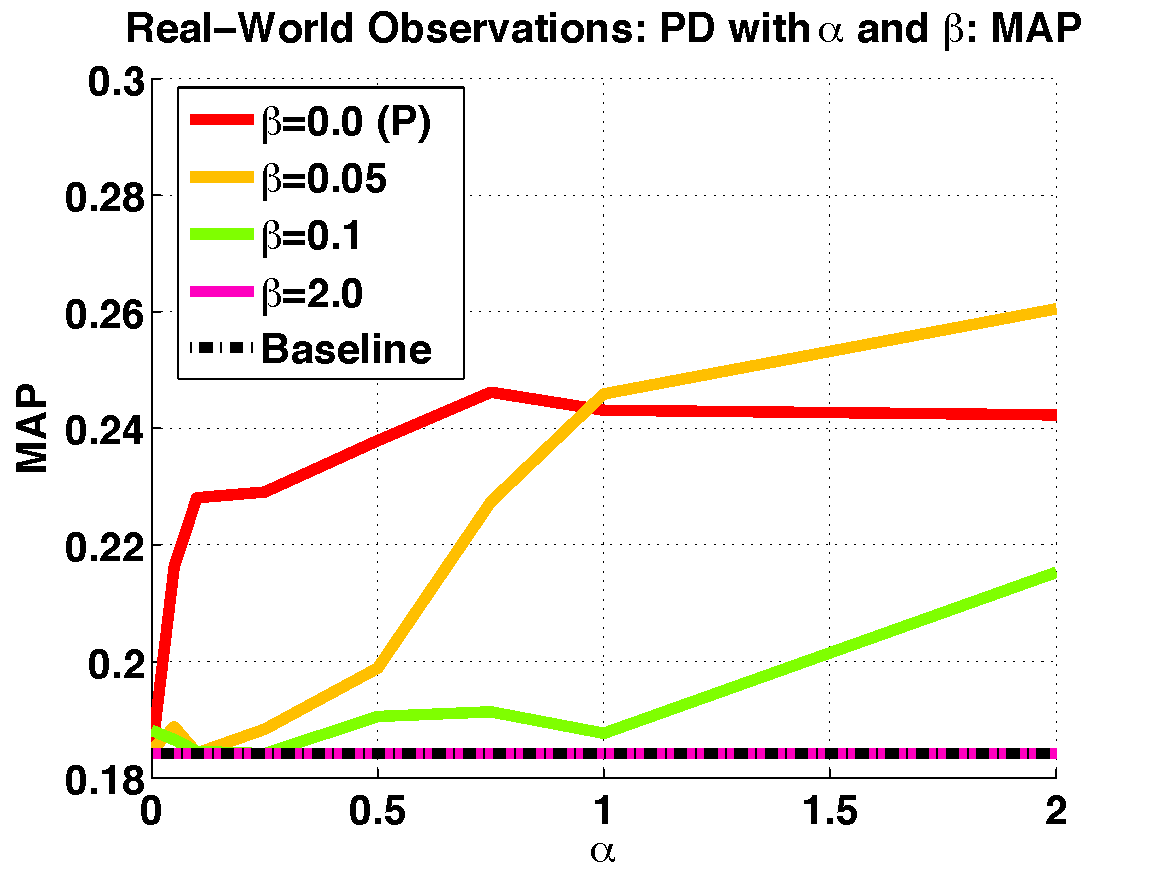
\includegraphics[width=0.5\textwidth]{pics/smucker/pd_map.pdf} & 
		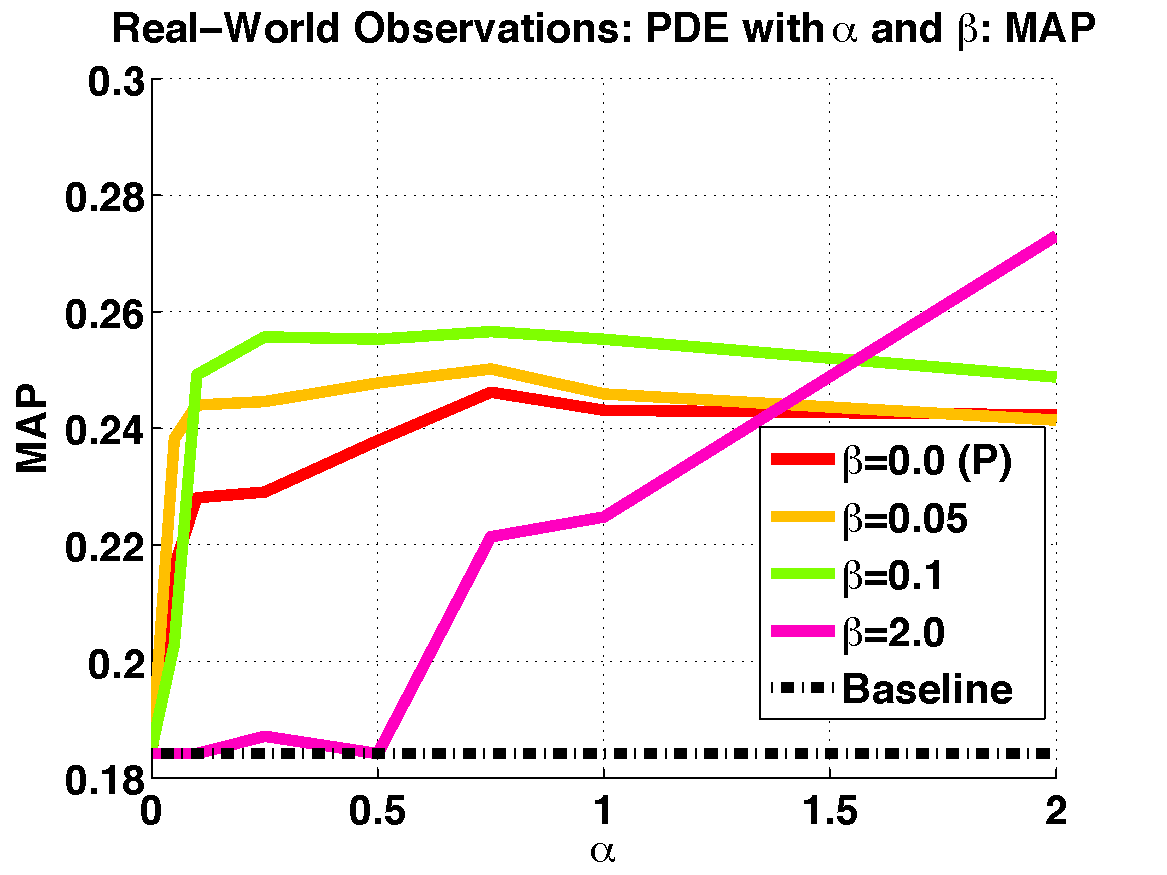
\includegraphics[width=0.5\textwidth]{pics/smucker/pde_map.pdf}
	 \\
		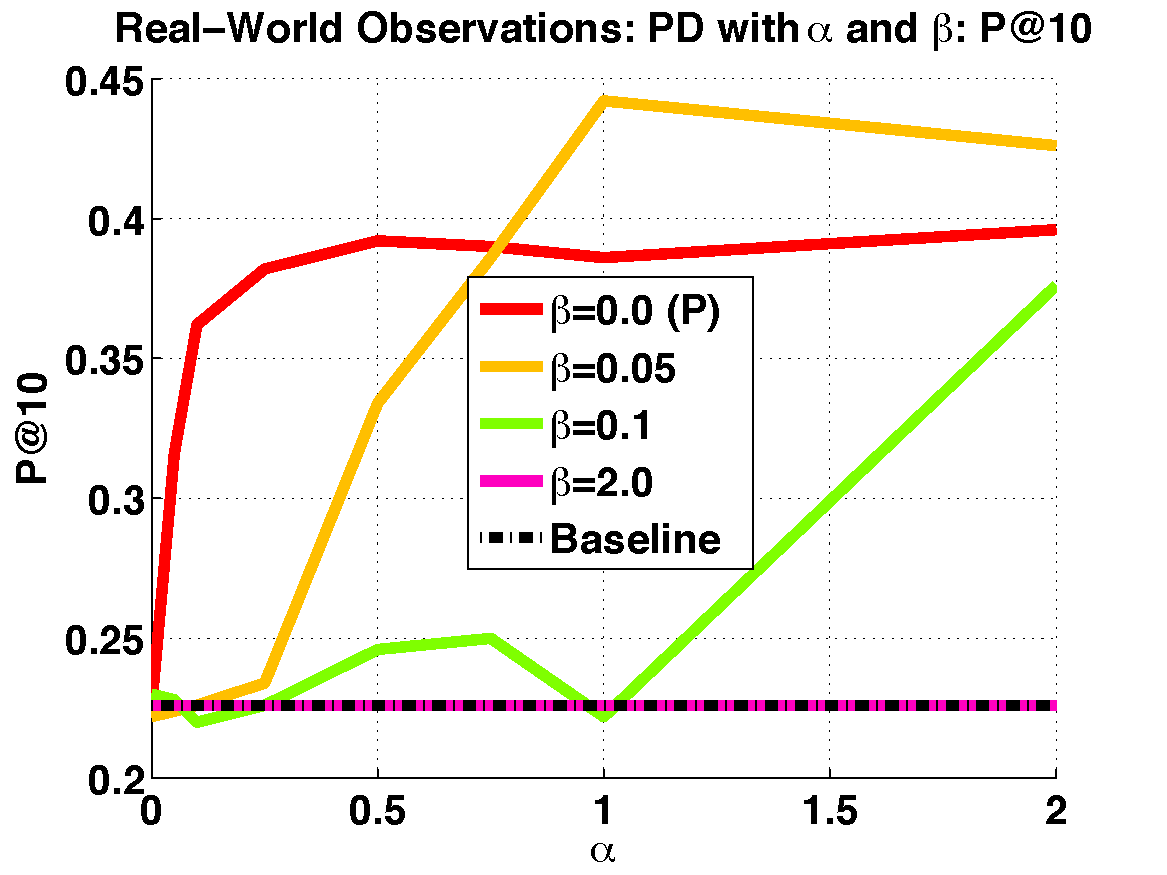
\includegraphics[width=0.5\textwidth]{pics/smucker/pd_p10.pdf} & 
		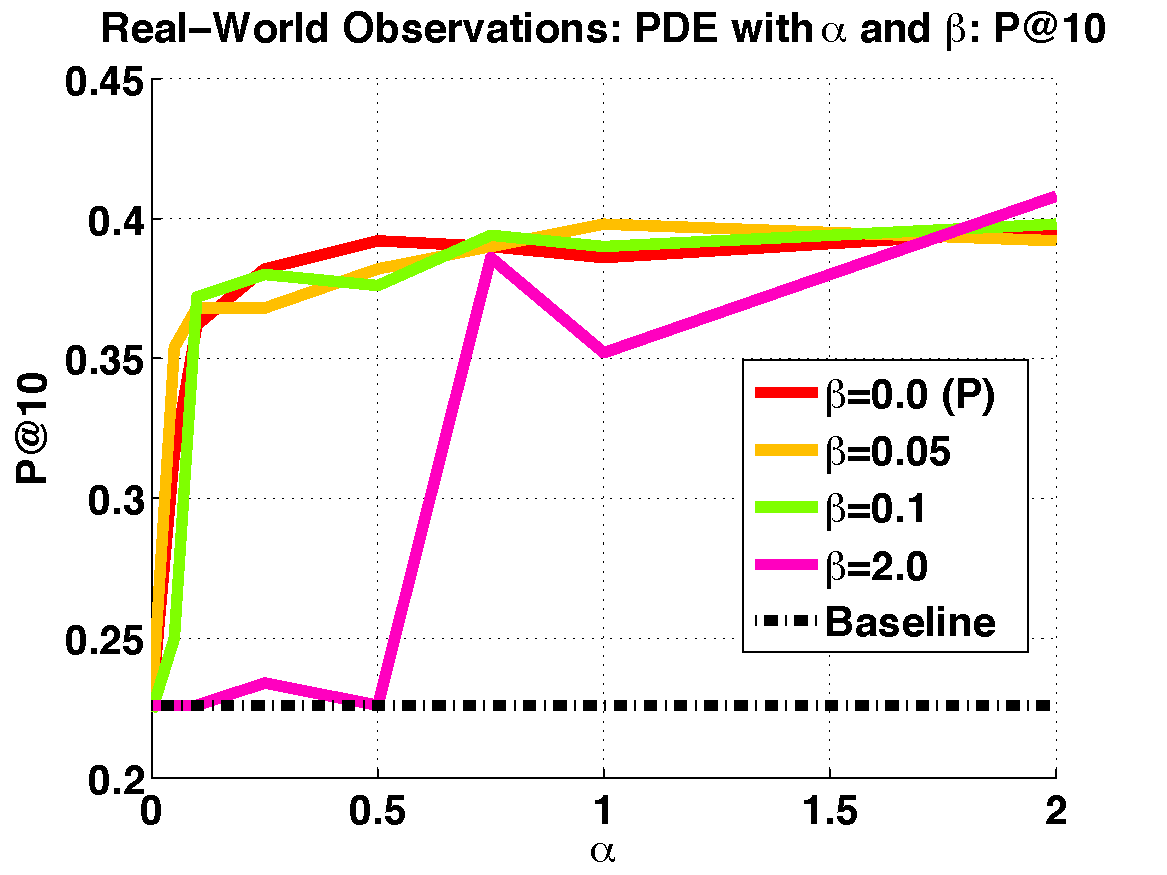
\includegraphics[width=0.5\textwidth]{pics/smucker/pde_p10.pdf}
	\end{array}
	$
	\caption{\textbf{Graphs illustrating performance (MAP and P@10) with variations in $\alpha$ and $\beta$. Graphs show performance for \emph{P} (red line), with variations in $\beta$ values for \emph{PD} and \emph{PDE}.}} \label{fig:noise:graphs}
\end{center}
\end{figure*}
%!TEX root = sigir2013site_clicks.tex
\section{Discussion and Conclusion}\label{sec_conclusion}
From our simulations discussed in Section \ref{sec_results}, we found several interesting features regarding the influences of clickthrough data on document rankings. We also observed several behavioural changes in clickthrough data when aspects such as noise and bias were introduced and adjusted. These observations allowed us to ascertain an understanding of the behaviour of clickthrough data, so often concealed within the `black box' of a machine-learned approach typically used in today's research.

\subsection{Summary of Findings}\label{sec:conclusion:summary}
Findings from our clickthrough simulations demonstrate a complex space, with many possible combinations and outcomes. Here, we briefly summarise our key findings regarding the behaviour of clickthrough data, and discuss the performance benefits observed.

We have ascertained that incorporating clickthrough data into search rankings has the potential to greatly improve performance. 
However, as a form of implicit relevance feedback, the performance gains that clickthrough data could potentially provide are severely limited through aspects such as noise (clicks on irrelevant documents) and bias (such as positional bias). To demonstrate the performance gains and losses observed, Table \ref{tbl:conclusion:summary} highlights performance figures obtained across all simulations run.

Under ideal conditions free from noise and bias, clickthrough data has the potential to make significant performance improvements over our baseline values. Indeed, under ideal conditions, model \textbf{PD} attained a MAP of 0.6269 over our baseline MAP of 0.1842. A P@10 value of 0.806 indicated that 8 out of 10 documents in the top 10 rankings were relevant - a huge improvement. As we began to factor in attributes such as noise and bias, we began to observe a drop in performance - as expected. However, our findings show that noise and bias can theoretically be overcome.

We showed that setting the probability of irrelevant clicks (noise, or $P(C|N)$) high enough will ensure that performance never improves upon baseline values. However, a more realistic value (between 0.25 and 0.5) was observed to allow for performance improvements similar - if not identical to - our `perfect world' simulations. However, as shown in Table \ref{tbl:conclusion:summary}, these improvements came after a much larger number of iterations. This therefore shows that irrelevant clicks can theoretically be overcome - more data is simply required to mitigate the effects that noise brings.

However, it is when positional bias was introduced that we observed perhaps the most significant drops in performance. Compared with a noise-only MAP of 0.6724, our recorded depth-proportional MAP was 0.5417. Depth-proportional or positional bias lowers the probability of a document being inspected the lower it is in the rankings. As such, documents at rank 30 have a 0.03\% chance of being examined. With an almost 0\% chance of being inspected, let alone clicked, positional bias severely affects the highest performance that can be attained. It can be said that further performance improvements could be attained over a greater number of iterations. However, such a value would be so high that there would be no advantage to site search engines.

Using parameters obtained from a real-world user study \cite{smucker2012time_based_calibration}, we still observed encouraging results. While MAP still improved from our baseline, it was significantly down on performance that was attained under ideal conditions. However, P@5 was doubled, with P@10 not far behind - showing that relevant documents were still percolating to the top of the rankings. It was clear that the probabilities used (especially of that for $P(C|N)$) hindered performance of our two more simplistic models, \textbf{P} and \textbf{PD}. \textbf{PDE} was able to offer improvements, demonstrating better tolerances.

\subsection{Discussion}\label{sec:conclusion:discussion}
Our findings have shown that there are noticeable variations in performance - both positive and negative - for even slight variations of parameters across the simulations that we ran. Specifically, our promotion and demotion weightings - $\alpha$ and $\beta$ - have been shown to be incredibly sensitive towards offering performance improvements or drops. Each model has demonstrated its own strengths and limitations, and it is clear from our findings that there is no simple `one-solution-fits-all' approach towards the issue of using clickthrough data to improve site search performance. Different sites will have different content and different users. While we acknowledge that using only the DOTGOV1 collection is a limitation, we hypothesise that our findings will generalise to other document collections. This issue is discussed in more detail in Section \ref{sec:conclusion:future}.

\begin{table}
	\renewcommand{\arraystretch}{1.3}
	\begin{center}
		\begin{small}
			\begin{tabularx}{\linewidth}{W{2cm}|W{1.1125cm}|W{1.1125cm}|W{1.1125cm}|W{1.1125cm}W{0.00000001cm}}
				
			 	& \centering{{\makebox[0pt][c]{\textbf{\emph{MAP}}}}} & \centering{\textbf{\emph{P@5}}} & \centering{{\makebox[0pt][c]{\textbf{\emph{P@10}}}}} & \centering{$i$}&
				\tabularnewline
				\hline
				
				\centering{\textbf{Baseline}}
				& \centering{0.1842}
				& \centering{0.272}
				& \centering{0.226}
				& \centering{N/A}&
				\tabularnewline[1.4em]
				\hline
				
				\centering{\textbf{Ideal}\\{\tiny\textbf{PD (0.75, 2.0)}}}
				& \centering{0.6727}
				& \centering{0.892}
				& \centering{0.81}
				& \centering{311}&
				\tabularnewline[1.4em]
				\hline
				
				\centering{\textbf{Depth}\\{\tiny\textbf{PD (0.75, 0.05)}}}
				& \centering{0.5417}
				& \centering{0.892}
				& \centering{0.778}
				& \centering{978}&
				\tabularnewline[1.4em]
				\hline
				
				\centering{\textbf{Noise}\\{\tiny\textbf{PD (0.75, 2.0)}}}
				& \centering{0.6724}
				& \centering{0.892}
				& \centering{0.81}
				& \centering{447}&
				\tabularnewline[1.4em]
				\hline
				
				\centering{\textbf{Noise/Depth}\\{\tiny\textbf{PD (0.75, 0.05)}}}
				& \centering{0.467}
				& \centering{0.836}
				& \centering{0.708}
				& \centering{994}&
				\tabularnewline[1.4em]
				\hline
				
				\centering{\textbf{Real-World}\\{\tiny\textbf{PDE (2.0, 2.0)}}}
				& \centering{0.273}
				& \centering{0.58}
				& \centering{0.408}
				& \centering{1935}&
				\tabularnewline[1.4em]
				
			\end{tabularx}
		\end{small}
	\end{center}
	\vspace{-0.3cm}
	\caption{\textbf{Table summarising the best performance observed across all simulations run. The model offering performance with the highlighted values - and associated $\alpha$ and $\beta$ values (in brackets) - are shown underneath each simulation's title.}\vspace{-0.5cm}}
	\label{tbl:conclusion:summary}
\end{table}

One of the disadvantages of clickthrough data is noise. Noise has been observed to degrade performance in the number of iterations required for a significant improvement to be observed. However, with the probability of a click on an irrelevant document set to a high value ($>=0.5$), no improvement whatsoever is observed. This is described as the performance `cliff' in Section \ref{sec:results:noise}. Therefore to yield good results, clickthrough data can contain noise; excessive amounts however will render the data as good as useless.

With the impact of noise, we also noticed a behavioural aspect of clickthrough data related to our demotion weighting parameter, $\beta$. With our `perfect world' simulations, we observed that performance improvements were only forthcoming with a small $\beta$ value - Figure \ref{fig:perfect_map_fall} illustrates this finding. However, by varying our relevant and irrelevant probabilities, $P(C|R)$ and $P(C|N)$, we discovered an intuitive link between $\beta$ and $P(C|R)$. The higher the $P(C|R)$, the more confident one could assume clicks were on relevant documents, hence a $\beta$ value would allow for higher performance to be attained in fewer iterations. Moreover, a lower $P(C|R)$ removed this confidence, and a smaller $\beta$ - such as those demonstrated to offer good improvements in Figure \ref{fig:perfect_map_fall} - would suffice. 

Bias - specifically positional bias - directly affects the number of iterations required for performance improvements to be observed, as discussed in Section \ref{sec:conclusion:summary}. This has a direct effect on site search due to the smaller number of users these search engines may experience compared to, for example, a commercial Web search engine. We found again that a slight variation in $\beta$ values could mitigate the effects of positional bias. A slightly higher $\beta$ value would give the demotion aspect of each model a greater chance to drop irrelevant documents down rankings.

There are many variations and permutations that can be selected. Not all are suited to site search scenarios. There are however several trade-offs that can be made. Each models offers its own advantages and disadvantages depending on the situation. For example, an environment with high quality data would be ideally suited to model \textbf{P}, and performance could theoretically be reached in a short time frame. Where precision is key, \textbf{PD} may be suited - but is not too robust. \textbf{PDE} has demonstrated an ability to provide an above-baseline improvement in performance, while tolerating higher levels of noise than the other two models. For any reasonable performance improvement, large volumes of clickthrough data are necessary due to the imperfections this form of data brings.

\subsection{Future Work}\label{sec:conclusion:future}
The research undertaken as part of this study has raised several interesting points that we feel warrant future work. Here, we address these points, discussing why undertaking them would be beneficial to the wider IR community.

Our first point regards the use of test collections. As previously discussed in Sections \ref{sec:method:materials} and above in Section \ref{sec:conclusion:discussion}, we ran our simulations with the TREC DOTGOV1 corpus only. This was regarded as a sensible decision due to the large volumes of data generated and limited space to report results. However, it would nevertheless be interesting to determine whether our findings hold for different collections of documents, or if adjustments must be made depending on factors such as the corpus size or genre. This issue raised also links into the idea of utilising a \emph{true} website's document collection in place TREC collections.

Secondly, we placed a cap on the maximum number of iterations that each of our simulations could run. Unfortunately, many of these simulations reached the maximum iteration count (see Tables \ref{tbl:results_perfect_view} and \ref{tbl:results_biased_demotion} for examples). This suggests that a greater level of performance could have been attained than we recorded, perhaps after several thousand iterations per simulation. Future work could remove such a cap and allow the simulations to reveal their true attainable maximum performance. This would allow for a better comparison between simulation results, and provide a better understanding of the volumes of data required to reach maximum performance.

With performance of our realistic simulations somewhat disappointing compared to our `perfect world' results, future work could investigate a series of models which are even more robust to factors of real-world clickthrough data, such as noise and different forms of bias. Finally, a form of machine-learned ranking approach would be beneficial as it would provide us with a meaningful set of results to compare our findings against.

Our findings have contributed to our understanding of clickthrough data, and what effects bias and noise have on such data. Results have provided an insight into what takes place inside a `black-box', machine-learned approach to optimising search engines when incorporating clickthrough data. Further investigation would allow us to improve our understanding of clickthrough data and how it can be used to improve search engine performance.

%\todo{=========LEIF'S COMMENTS========}
%remove p graphs, put red line in the other four and say that this is P's performance.
%just have 0.0, 0.1, 0.25, 2.0. take out stuff in the middle, makes it look cluttered.

%perhaps readjust size of graphs, make them as big as possible.

%in the tables, try remove the redundancy - i.e. remove the PD, PDE stuff...
%a row for PD, a row for PDE so it removes the PD/PDE duplications...

%can performance of 0.1840 with i = 1000 be shortened to something like 1.84 (1000)???

{\bf Acknowledgements.} First, I would like to thank Colin Wilkie (\href{http://www.twitter.com/kojayboy}{\emph{@kojayboy}}) for his friendship and comments on my work throughout this project. I would like to thank Dr. Gethin Norman for his understanding during what has been a very challenging year. However, I would like to extend my deepest gratitude to my supervisor, Dr. Leif Azzopardi (\href{http://www.twitter.com/leifos}{\emph{@leifos}}). Without his friendship, support and guidance, I certainly would not have crossed the finish line I was beginning to think I'd never reach. Thank you.

\bibliographystyle{abbrvnat}
\small{\bibliography{sigproc,cikm2013site_clicks}}
\balancecolumns

\end{document}
